\newpage

\section{Implementation Details}
\label{app:implementation}

Code for the agent and multi-task environments used in our experiments is available on GitHub at \href{https://github.com/UT-Austin-RPL/amago}{UT-Austin-RPL/amago}.


\paragraph{Base RL Details.} We focus on evaluating changes to the training objective of long-term memory policies trained by off-policy actor-critic updates. Our implementation makes use of many orthogonal technical details from AMAGO \cite{grigsby2024amago}. In the context of this work, the most important detail is the use of a global (task-agnostic) PopArt \cite{hessel2019multi} layer to normalize $Q$-values \textit{of the ``dependent'' update} ($\mathcal{L}_{\text{Actor}}, \mathcal{L}_{\text{Critic}}$), which brings loss functions to a predictable absolute scale but does not change the fact that each task has different relative values. Trying to compare learning updates while skipping this technique would make the $Q$-dependent baselines far too reliant on accurate grid-searches of optimization hyperparameters across domains. Table \ref{tbl:rl_hparams} provides the list of hyperparameters used in our main experiments. All of the results in this paper were completed on NVIDIA A5000 GPUs. We train each agent on one GPU whenever possible but add a second GPU for Procgen Memory-Hard (Figure \ref{fig:procgen_memory}) where model size and context length use all available memory.

\begin{table}[h!]
\resizebox{\textwidth}{!}{\begin{tabular}{@{}lcccccc@{}}
\toprule
                                  & \textbf{Meta-World} & \textbf{POPGym}          & \textbf{Procgen Easy} & \textbf{Procgen Memory-Hard} & \textbf{Atari} & \textbf{BabyAI} \\ \midrule
Learning Rate                     & 5e-4                & 1e-4                     & 1e-4                  & 1e-4                         & 1e-4           & 1e-4                 \\
Batch Size (In Sequences)         & 24                  & 24                       & 24                    & 16                           & 32             & 24                   \\
Replay Buffer Size (in Timesteps) & 8M                  & 15,000 Full Trajectories & 18M                   & 80M                          & 8M            & 10M                  \\
L2 Penalty                        & 1e-4                & 1e-4                     & 5e-3                  & 5e-3                         & 5e-3           & 1e-3                 \\
Grad Clip (Norm)                  & 2                   & 1                        & 1                     & 1                            & 1              & 1                    \\
Learning Update $\gamma$         & \multicolumn{6}{c}{$[0.1, .9, .95, .97, .99, .995, .999]$}                                                                                    \\
Rollout $\gamma$                  & \multicolumn{6}{c}{.999}                                                                                                                      \\
Critic Ensemble Size              & \multicolumn{6}{c}{4}                                                                                                                         \\
Target Network Update $\tau$      & \multicolumn{6}{c}{.003}                                                                                                                      \\ \bottomrule
\end{tabular}}
\caption{\textbf{Learning Hyperparameter Details.}}
\label{tbl:rl_hparams}
\end{table}


\paragraph{Model Architectures.} All of our experiments use causal Transformers trained with the AdamW optimizer \cite{loshchilov2017decoupled}. We apply Normformer \cite{shleifer2021normformer} and $\sigma$Reparam \cite{zhai2023stabilizing} with Leaky ReLU activations to all architectures. These details are intended to stabilize the policy against long training runs of millions of gradient steps but are applicable to any sequence modeling problem; our results did not require any changes that are specific to RL. We use fixed (sinusoidal) position embeddings \cite{vaswani2017attention}. Table \ref{tbl:arch_hparams} lists Transformer architectural details for each of our main experiments. The ``timestep encoder'' maps the potentially multi-modal meta-RL inputs of observations, actions, rewards, and reset signals to a fixed-size vector (Figure \ref{fig:arch}). State-based domains (Meta-World and POPGym) can concatenate and merge this information with a small feed-forward network. In pixel-based environments, we first embed the image observation with a CNN. We evaluated both the small ``Nature'' architecture \cite{mnih2015human} and the residual IMPALA CNN \cite{espeholt2018impala}. Our results default to IMPALA with additional Group Normalization \cite{wu2018group, kumar2022offline}. We apply the random pad and crop data augmentation from DrQV2 \cite{yarats2021mastering} to Procgen and Atari experiments. Image features extracted by the CNN are normalized before being added to action, reward, and terminal data. For consistency with the rest of the architecture we use LayerNorm \cite{ba2016layer}. Preliminary experiments found many of these vision details to be flexible.

\begin{table}[h!]
\resizebox{\textwidth}{!}{\begin{tabular}{@{}lcccccc@{}}
\toprule
                           & \textbf{Meta-World} & \textbf{POPGym} & \textbf{Procgen Easy}                                                              & \textbf{Procgen Memory-Hard}                                                       & \textbf{Atari}                                                                     & \textbf{BabyAI}                                                               \\ \midrule
Timestep Encoder           & FF (512, 256)       & FF (512, 200)   & \begin{tabular}[c]{@{}c@{}}IMPALA CNN\\ {[}16, 32, 32{]} block depths\end{tabular} & \begin{tabular}[c]{@{}c@{}}IMPALA CNN\\ {[}20, 36, 64{]} block depths\end{tabular} & \begin{tabular}[c]{@{}c@{}}IMPALA CNN\\ {[}16, 32, 32{]} block depths\end{tabular} & \begin{tabular}[c]{@{}c@{}}Multi-Modal\\CNN (Grid), RNN (Language), FF (Other) \end{tabular} \\
Transformer Dim.           & 320                 & 256             & 512                                                                                & 512                                                                                & 256                                                                                & 256                                                                                \\
Transformer FF Dim.        & 1280                & 1024            & 2048                                                                               & 2048                                                                               & 1024                                                                               & 1024                                                                               \\
Transformer Layers         & 3                   & 3               & 3                                                                                  & 6                                                                                  & 3                                                                                  & 4                                                                                  \\
Transformer Heads          & 8                   & 8               & 8                                                                                  & 8                                                                                  & 8                                                                                  & 8                                                                                  \\
Context Length (Timesteps) & 256                 & 600             & 128                                                                                & 768                                                                                & 64                                                                                 & 512                                                                                 \\
Actor and Critic MLPs      & (256, 256)          & (256, 256)      & (256, 256)                                                                         & (256, 256)                                                                         & (256, 256)                                                                         & (256, 256)                                                                         \\
Critic Output Bins (Ind.)  & 128                 & 64              & 128                                                                                & 128                                                                                & 128                                                                                & 32                                                                                \\ \bottomrule
\end{tabular}}
\caption{\textbf{Agent Architecture Details.}}
\label{tbl:arch_hparams}
\end{table}

\begin{figure}[h!]
    \centering
    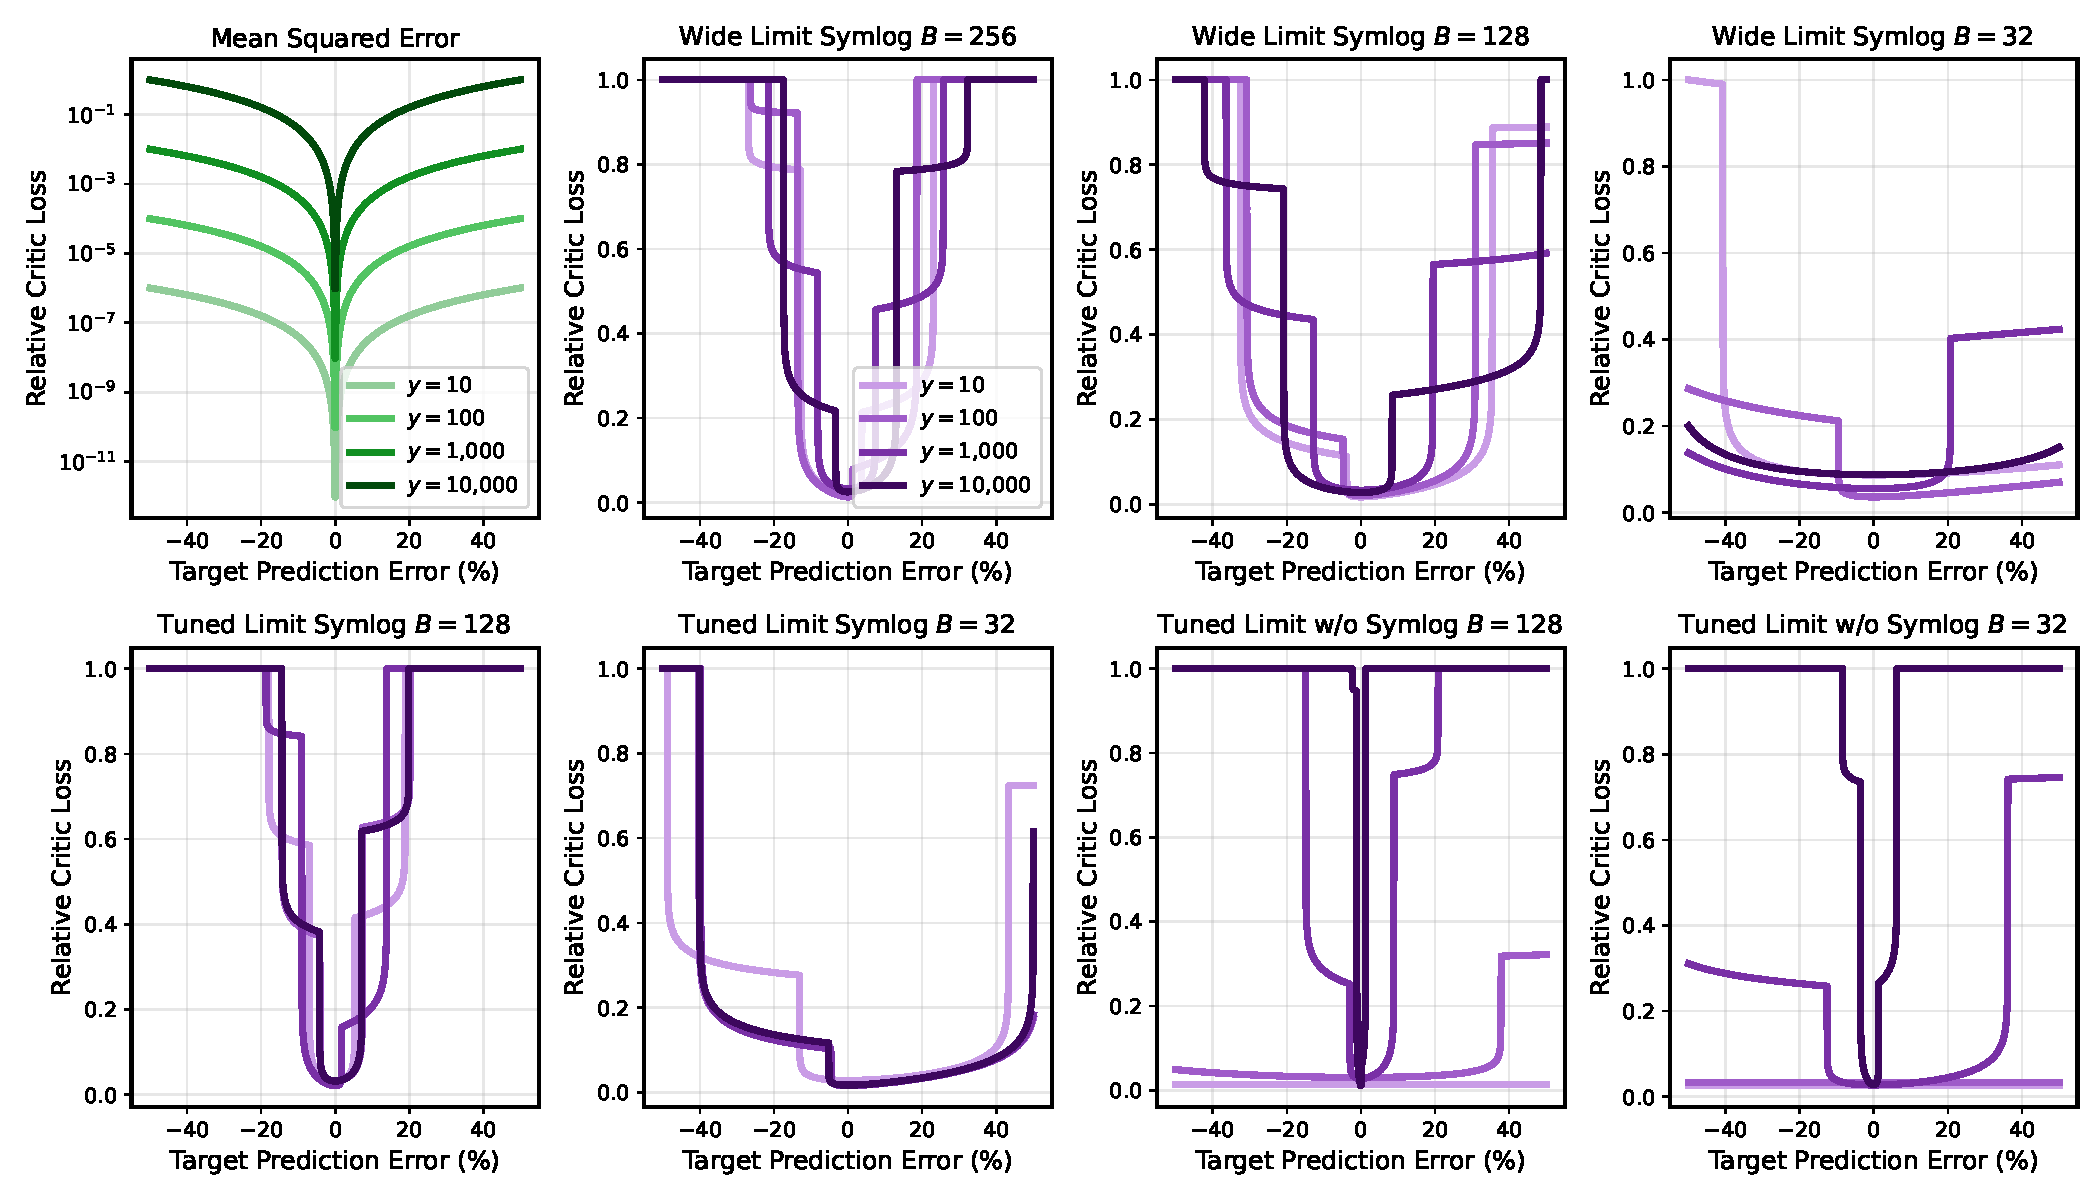
\includegraphics[width=\textwidth]{figures/final/twohot_prediction_error.pdf}
    \caption{\textbf{Scale-Resistant Regression.} We plot the critic loss as a function of the \textit{relative} prediction error of the value target ($y$) across several orders of magnitude. Standard MSE (top left) assigns significantly different weights to the same relative inaccuracy across tasks according to the absolute value of their current targets. Converting regression to classification can map a wide range of values to a similar loss, but this effect can benefit from tuning. We show $7$ different strategies. ``Wide Limit'' refers to the DreamerV3 approach of setting extreme $(R_\text{low}, R_\text{high})$ defaults that do not need tuning. ``Tuned Limit`` bins set the upper and lower bound close to the expected range for the domain (in this example: $[-100, 15,000]$).}
    \label{fig:relative_losses_extended}
\end{figure}



\paragraph{Value Classification Details.} We convert value regression (Equation \ref{eq:critic_dep}) to classification (Equation \ref{eq:critic_ind}) by creating labels for $B$ return bins $\mathbf{b} = [b_0, b_1, \dots, b_B]$. Bins are typically spaced at fix intervals between pre-defined upper and lower bounds on the return $(b_0 = R_\text{low}, b_B = R_\text{high})$. The critic network ($Q_B$) outputs (softmax) probabilities over these bins, and its value prediction can be recovered by $Q(h_t, a_t) = Q_B(h_t, a_t)^\mathsf{T}\mathbf{b} $.  A scalar temporal difference target $y$ is mapped to a classification label by $\text{twohot}_B: \mathbb{R} \rightarrow [0, 1]^{B}$ --- a function that outputs zeroes everywhere aside from two consecutive indices corresponding to the closest bin below $y$ ($b_{i-1}$) and above $y$ $(b_{i}$), which are filled based on their distance from $y$:

\begin{minipage}{0.45\textwidth}
  \begin{align}
    \text{twohot}_B(y)[i-1] = \frac{y - b_{i-1}}{b_i - b_{i-1}}
    \end{align}
\end{minipage}
\begin{minipage}{0.45\textwidth}
    \begin{align}
    \text{twohot}_B(y)[i] = \frac{b_{i} - y}{b_i - b_{i-1}}
    \end{align}
\end{minipage}


Therefore there are two main settings to configure for each experiment: 1) the bin limits $[R_\text{low}, R_\text{high}]$, and 2) the number of (evenly spaced) bins between the limits, $B$. We can often set bin limits using prior knowledge of the maximum and minimum return in a given domain, but it can be challenging to establish correct settings for a new application or reward function. The number of bins $B$ defines the ``resolution'' of the critic network. Using fewer bins puts more emphasis on outputting correct label weights while adding more bins shifts focus to outputting correct label indices. This trade-off is interesting because it is somewhat unusual for the label space of a classification problem to be a tunable hyperparameter; for example, the dataset determines the number of labels in object recognition or language modeling. Figure \ref{fig:bin_comparison} provides two single-task examples where lower label counts are more sample efficient, and Figure \ref{fig:procgen_analysis} in the main text supports a similar conclusion in multi-task Procgen. These settings can be easily adjusted in our open-source code, but their trade-offs are underexplored in the results of this work. Instead, we focus on reducing tuning by following details in DreamerV3 \cite{hafner2023mastering}. We set $[R_\text{low}, R_\text{high}]$ extremely wide such that they capture the full range of every experiment and do not need to be tuned. We transform $y$ with ``symlog'' before label creation:
$\text{twohot}_B(y) \leftarrow \text{twohot}_B(\text{symlog(y)})$. Scalar values are recovered from bin probabilities by inverting this transformation with ``symexp'': $Q(h_t, a_t) = \text{symexp}(Q_B(h_t, a_t)^\mathsf{T}\mathbf{b})$, where:

\begin{minipage}{0.45\textwidth}
  \begin{align}
    \text{symlog}(y) = \text{sign}(y) \ln(|y| + 1)
    \end{align}
\end{minipage}
\begin{minipage}{0.45\textwidth}
    \begin{align}
    \text{symexp}(b) = \text{sign}(b) (\exp(|b|) - 1)
    \end{align}
\end{minipage}



Bins are spaced evenly between $b_0 = \text{symlog}(R_\text{low})$ and $b_B = \text{symlog}(R_\text{high})$. This symlog trick skews labels to give more resolution to smaller return values while retaining our ability to represent extreme outliers at a lower resolution. In general, we find that setting a wide limit $(R_\text{low},  R_\text{high})$, increasing the label count $B$, and compressing labels with symlog/symexp is the safest way to achieve scale-invariance across domains (Section \ref{sec:method}). An example is illustrated by Figure \ref{fig:relative_losses_extended}. We always use symlog and wide limits of $(R_\text{low} = -1e5, R_\text{high} = 1e5)$, and only tune the bin count $B$ (Table \ref{tbl:arch_hparams}). However, it is likely that sample efficiency can be improved by tuning bin counts, limits, and the use of the symlog transform for each individual domain. Figure \ref{fig:symlog_comparison} illustrates the trade-off between bin counts and symlog with tuned return limits in a single-task setting.

\begin{figure}[h!]
    \centering
    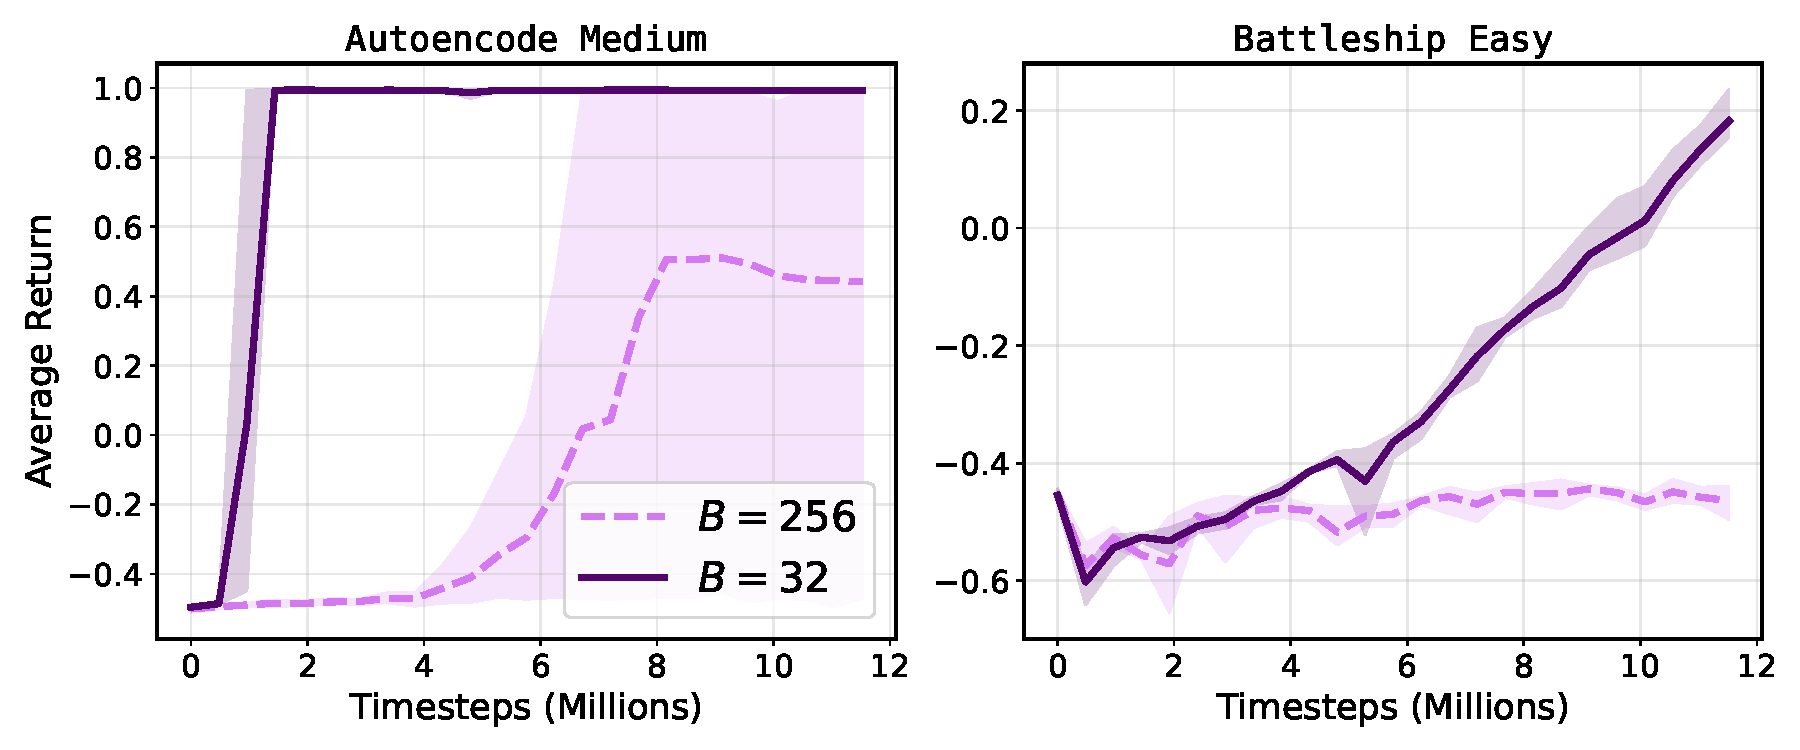
\includegraphics[width=0.8\linewidth]{figures/final/bin_comparison_popgym.pdf}
    \caption{\textbf{Bin Counts in POPGym.} We compare two label space sizes ($B$) with the same $R_\text{low}$ and $R_\text{high}$ limits on two single-task POPGym environments \cite{morad2023popgym}.}
    \label{fig:bin_comparison}
\end{figure}

\begin{figure}[h!]
    \centering
    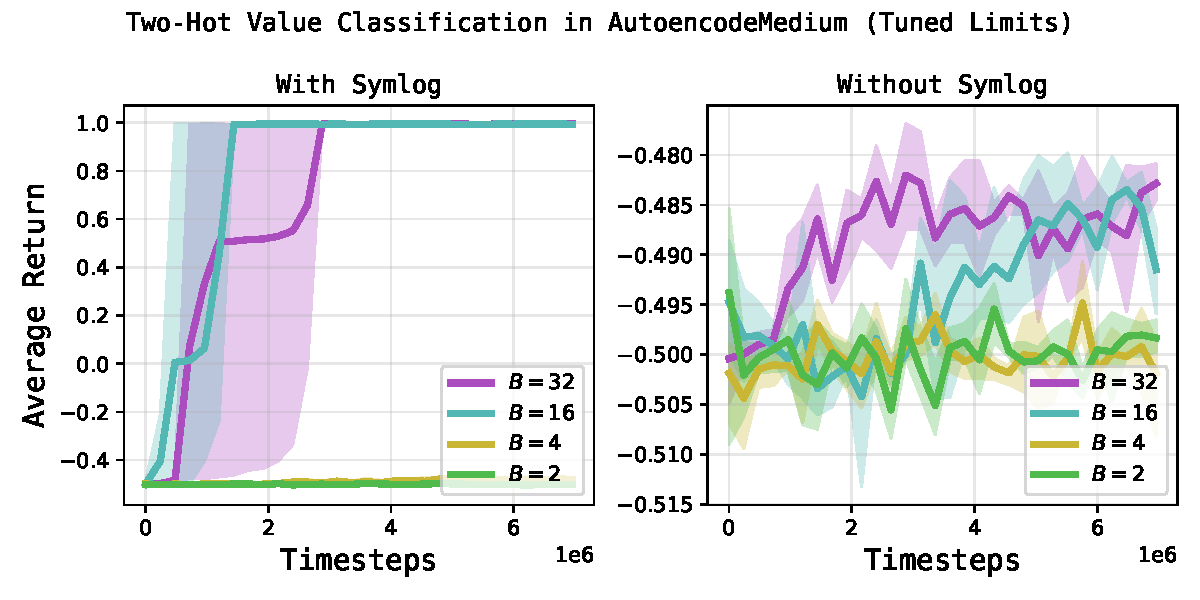
\includegraphics[width=0.8\linewidth]{figures/final/symlog_vs_no_symlog_appendix.pdf}
    \caption{\textbf{Symlog and Bins with Tuned Limits.} We would expect a decrease in the number of value bins to increase sample efficiency up until a point where each bin covers too broad a value range to learn accurate targets. We demonstrate this with a POPGym task \cite{morad2023popgym}. These experiments multiply every reward by $\times 100$ during training and set bin limits of $R_{\text{low}} = -110, R_{\text{high}} = 110$. Shaded areas indicate the maximum and minimum value of three trials.}
    \label{fig:symlog_comparison}
\end{figure}


\section{Additional Environment Details}

\paragraph{Multi-Task POPGym.} The environment samples uniformly between $27$ POPGym \cite{morad2023popgym} tasks with discrete actions where both the action space and observation space have dimension $< 30$. A full list is provided as part of Figure \ref{fig:popgym_learning_curves}. The cutoff of dimension $30$ is arbitrary but some limit is necessary because POPGym has several tasks with unusually large action spaces. We are then able to create unified input and output spaces by padding observations and actions to dimensions of $26$. If the agent selects an action index that is not valid for the current task, the environment samples a valid action uniformly at random. An additional observation feature indicates whether the previous action was valid. The one-shot evaluation setting is implemented as in E-RL$^2$ \cite{stadie2018some}, where rewards for the exploration episode are inputs to the policy but are not allowed to become true reward outputs that are optimized by RL updates.

\paragraph{Multi-Game Procgen.} We merge individual Procgen \cite{cobbe2020leveraging} games into a multi-task environment by randomly sampling a new game between meta-rollouts. The same procedurally generated level is then played twice before a new game and level are sampled. In order to allow policies without long-term memory to form accurate value estimates, we draw a small black box in the top left corner of the screen throughout the second episode. We enforce a maximum rollout length (across both episodes) of $H=2500$ for the $5$-game easy mode (Figure \ref{fig:popgym_easy_mode}) and $H=5000$ for the memory-hard mode (Figure \ref{fig:procgen_memory}). In memory-hard mode, we sample levels from the ``memory'' distribution when available and ``hard'' otherwise. The memory distribution extends the hard difficulty by introducing partial observability. Memory mode was not evaluated in the original Procgen results and has been rarely used since. Therefore the results in Figure \ref{fig:procgen_memory} are normalized according to the established scale for hard mode. With the exception of the ``Miner'' game, these upper bound scores transfer to memory mode as it does not adjust the problem difficulty but does hide information about the layout of the level.
\begin{wrapfigure}{r}{.45\textwidth}
\vspace{-12mm}
\begin{center}
    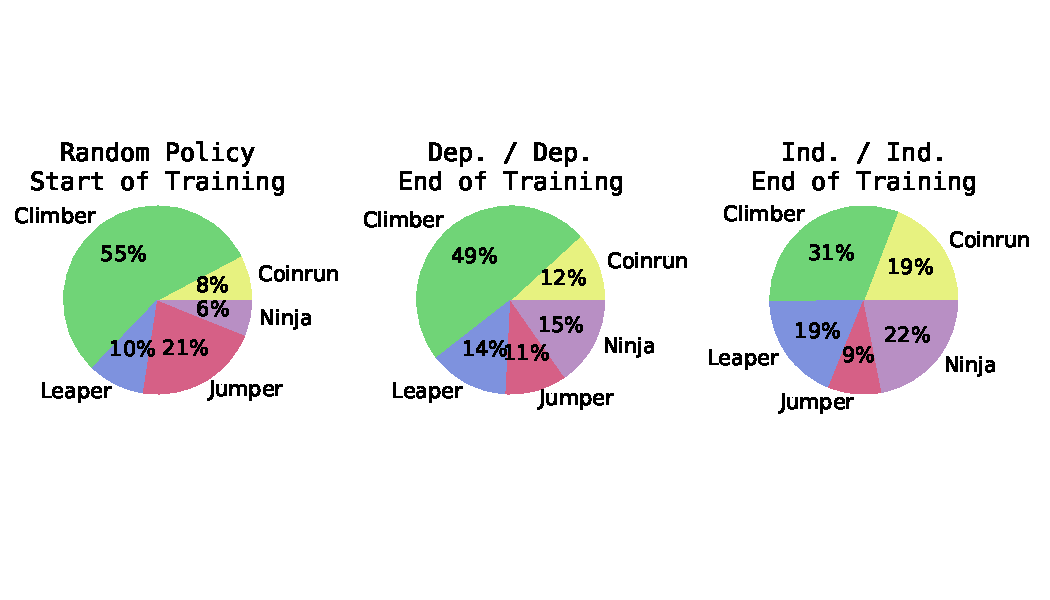
\includegraphics[width=.43\textwidth]{figures/final/procgen_frame_count_pie_chart.pdf}
    \vspace{-12mm}
    \caption{\textbf{Imbalanced Procgen Datasets.} We measure the inflow of experience to the replay buffer by game. Climber accounts for much of our early training data but the buffer is rebalanced as policies improve.}
    \label{fig:procgen_frame_counts}
    \vspace{-8mm}
\end{center}
\end{wrapfigure}

One detail is that selecting a random game between resets does not account for the length of each rollout or the way episode length increases or decreases as the agent improves. As a result, our multi-task Procgen experiments create imbalanced datasets where each game makes up an uneven amount of incoming training data (Figure \ref{fig:procgen_frame_counts}). We consider this to be an interesting additional challenge that off-policy methods with large replay buffers are well suited to address.


\paragraph{Atari.} We select $10$ games that do not involve challenging exploration but that have human-level returns on several different orders of magnitude. The list of games is included in Figure \ref{fig:atari_result}. We use the standardized $\texttt{v5}$ variants of the Atari environments in Gymnasium \cite{towers_gymnasium_2023}. In addition to removing reward clipping, we do not use frame stacking or greyscaling. Instead, agents can learn short-term state estimation and task identification from context sequences of RGB frames.

\paragraph{BabyAI.} BabyAI provides the agent with a $7 \times 7$ partial view of its surroundings in a procedurally generated gridworld. Goals are communicated with relatively simple language instructions, which we represent as sequences from a vocabulary of $29$ tokens. Each reset randomly samples a new goal type and gridworld generation strategy from $50$ tasks in the \href{https://minigrid.farama.org/environments/babyai/}{Minigrid registry} during training, and $18$ tasks during testing. A full list of task names is included as part of Figure \ref{fig:babyai_icrl}.


\section{Additional Results}
\label{app:results}
\label{app:popgym}

Large figures displaying results from each task in our POPGym (Figure \ref{fig:popgym_learning_curves}) and BabyAI (Figure \ref{fig:babyai_appendix}) experiments are listed on the following two pages. These figures are followed by learning curves for each Meta-World ML45 task.


\begin{figure}[h!]
    \centering
    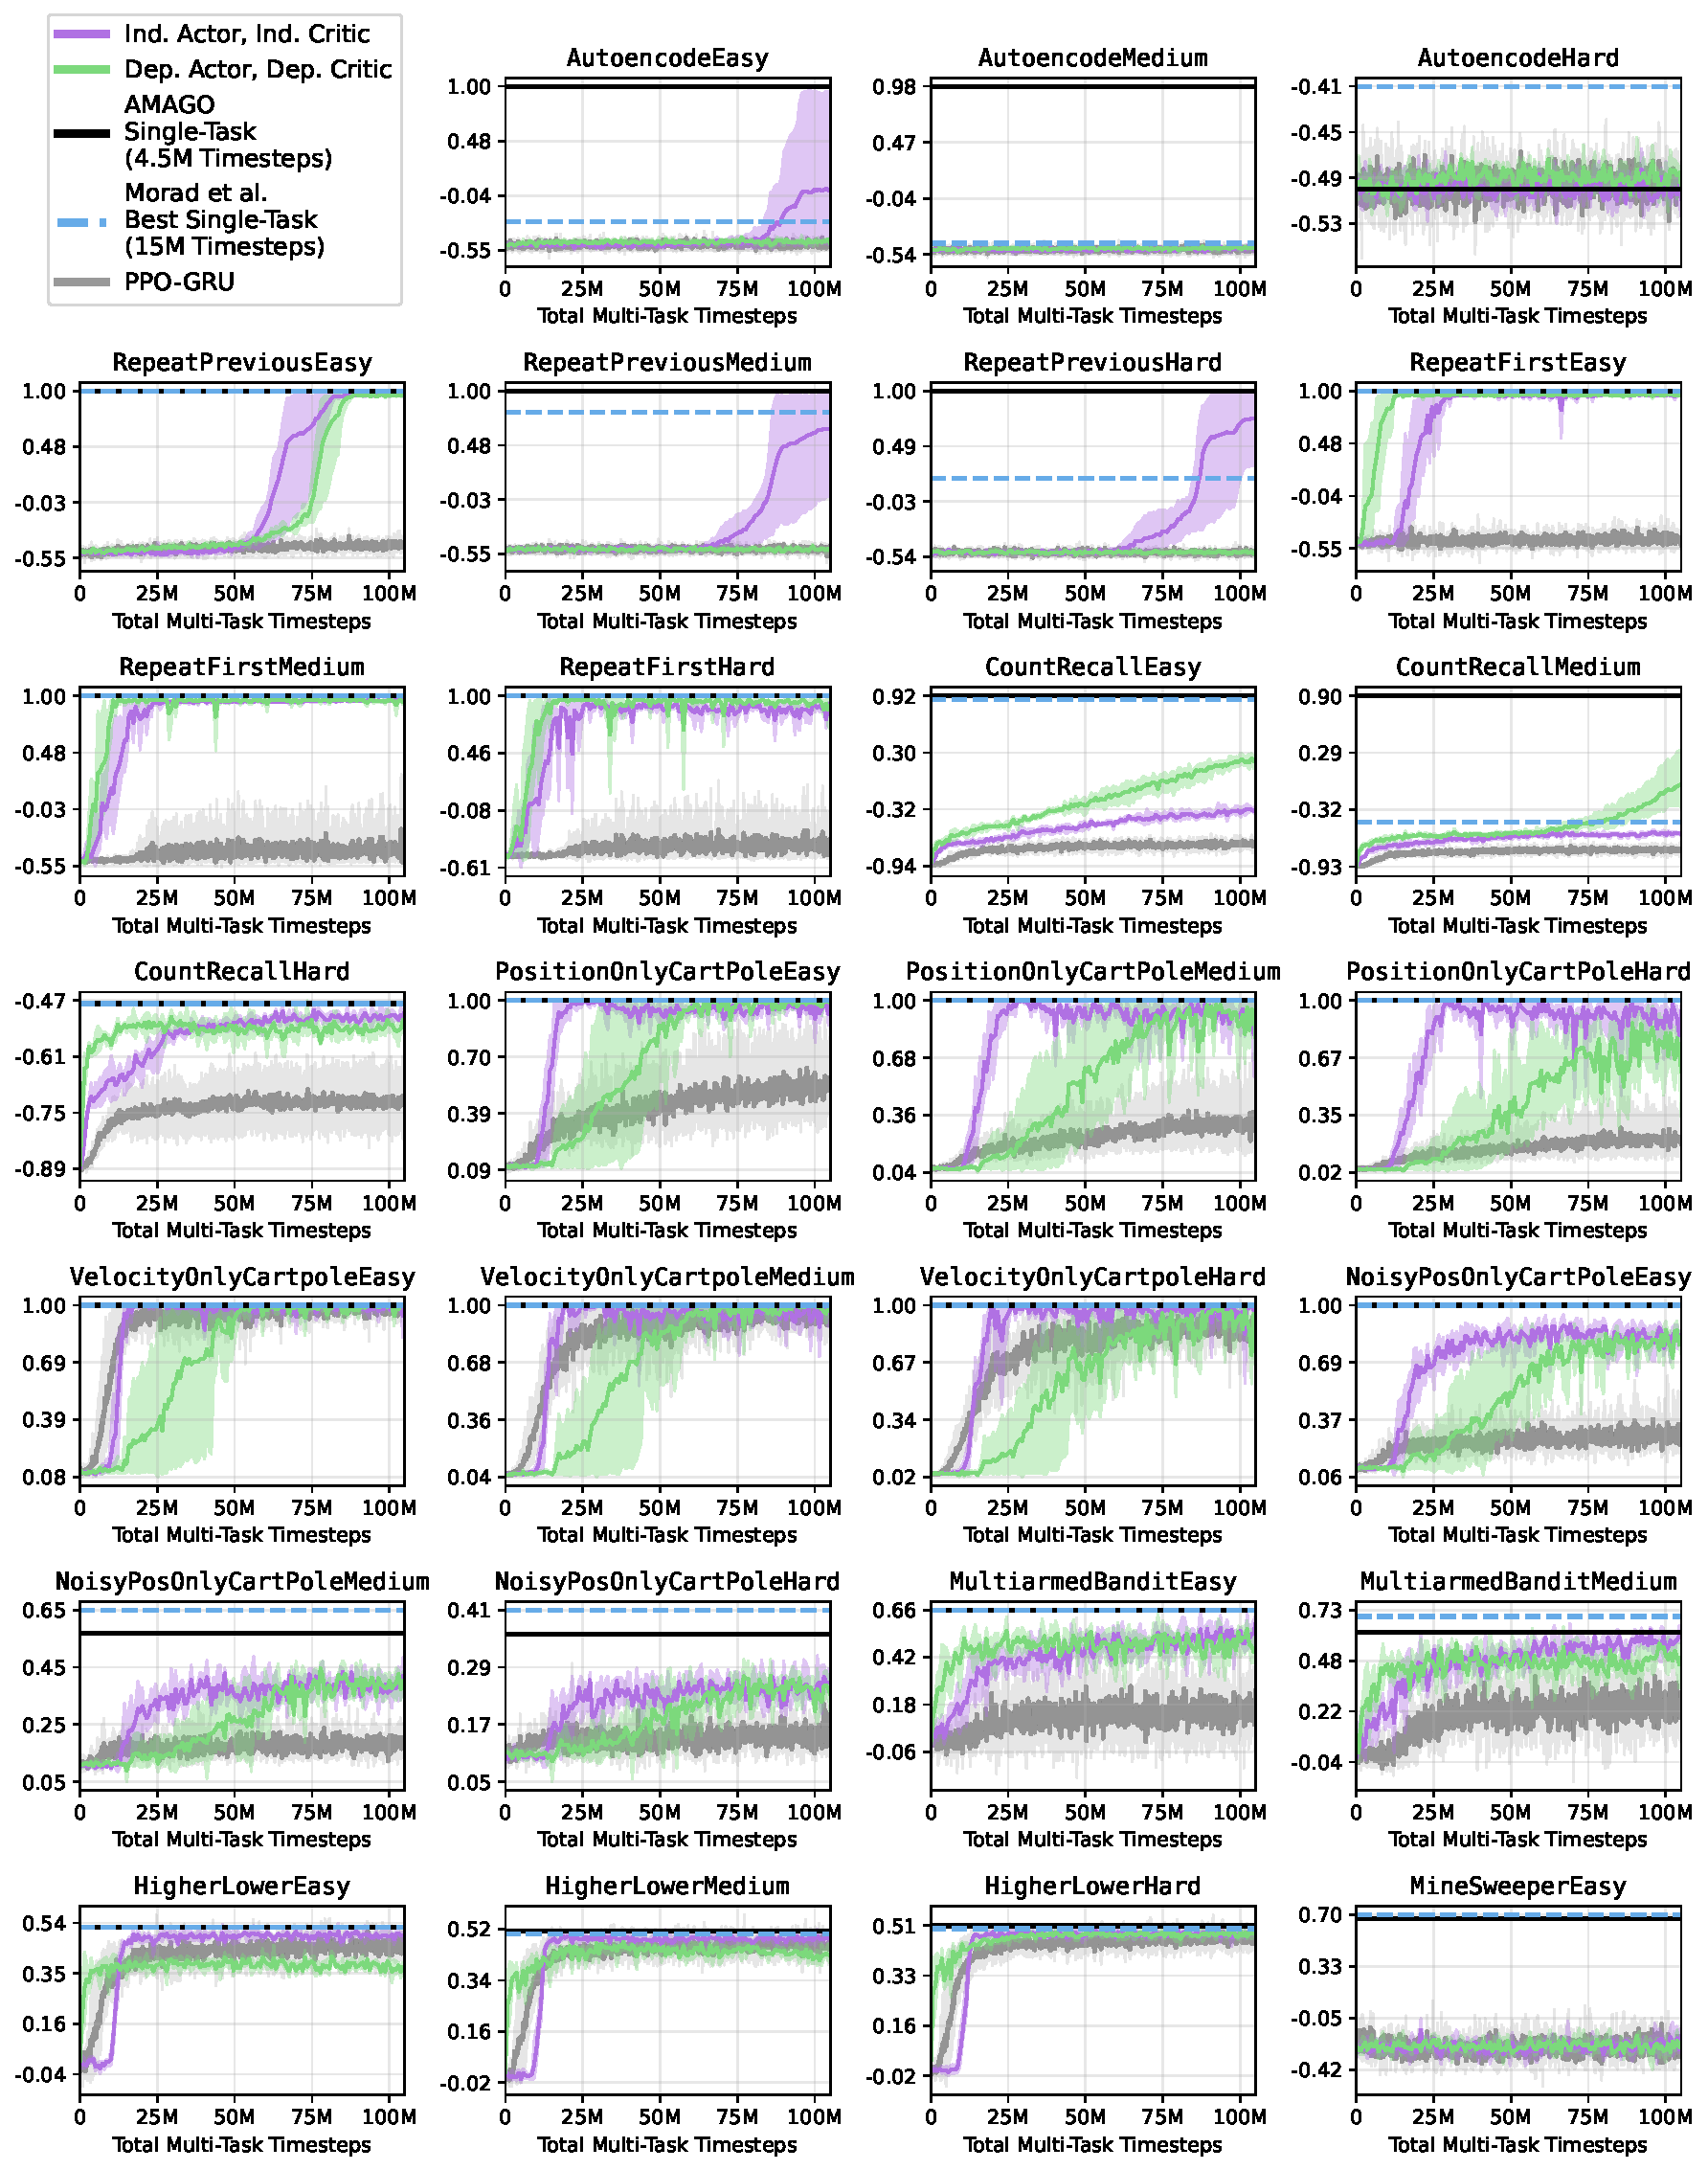
\includegraphics[width=\textwidth]{figures/final/popgym_appendix_learning_curves_final.pdf}
    \caption{\textbf{One-Shot Multi-Task POPGym.} Plotted on the raw scale of returns in each environment. Error bars denote the maximum and minimum results over three trials. Single-Task reference scores at 15M timesteps indicate the best of 14 sequence model backbones trained by PPO in the results of Morad et al. \cite{morad2024reinforcement}. AMAGO \cite{grigsby2024amago} single-task reference scores are taken at $4.5$M timesteps, which is a safe upper-bound on the timesteps encountered for each task during multi-task training.}
    \label{fig:popgym_learning_curves}
\end{figure}

\begin{figure}[h!]
    \centering
    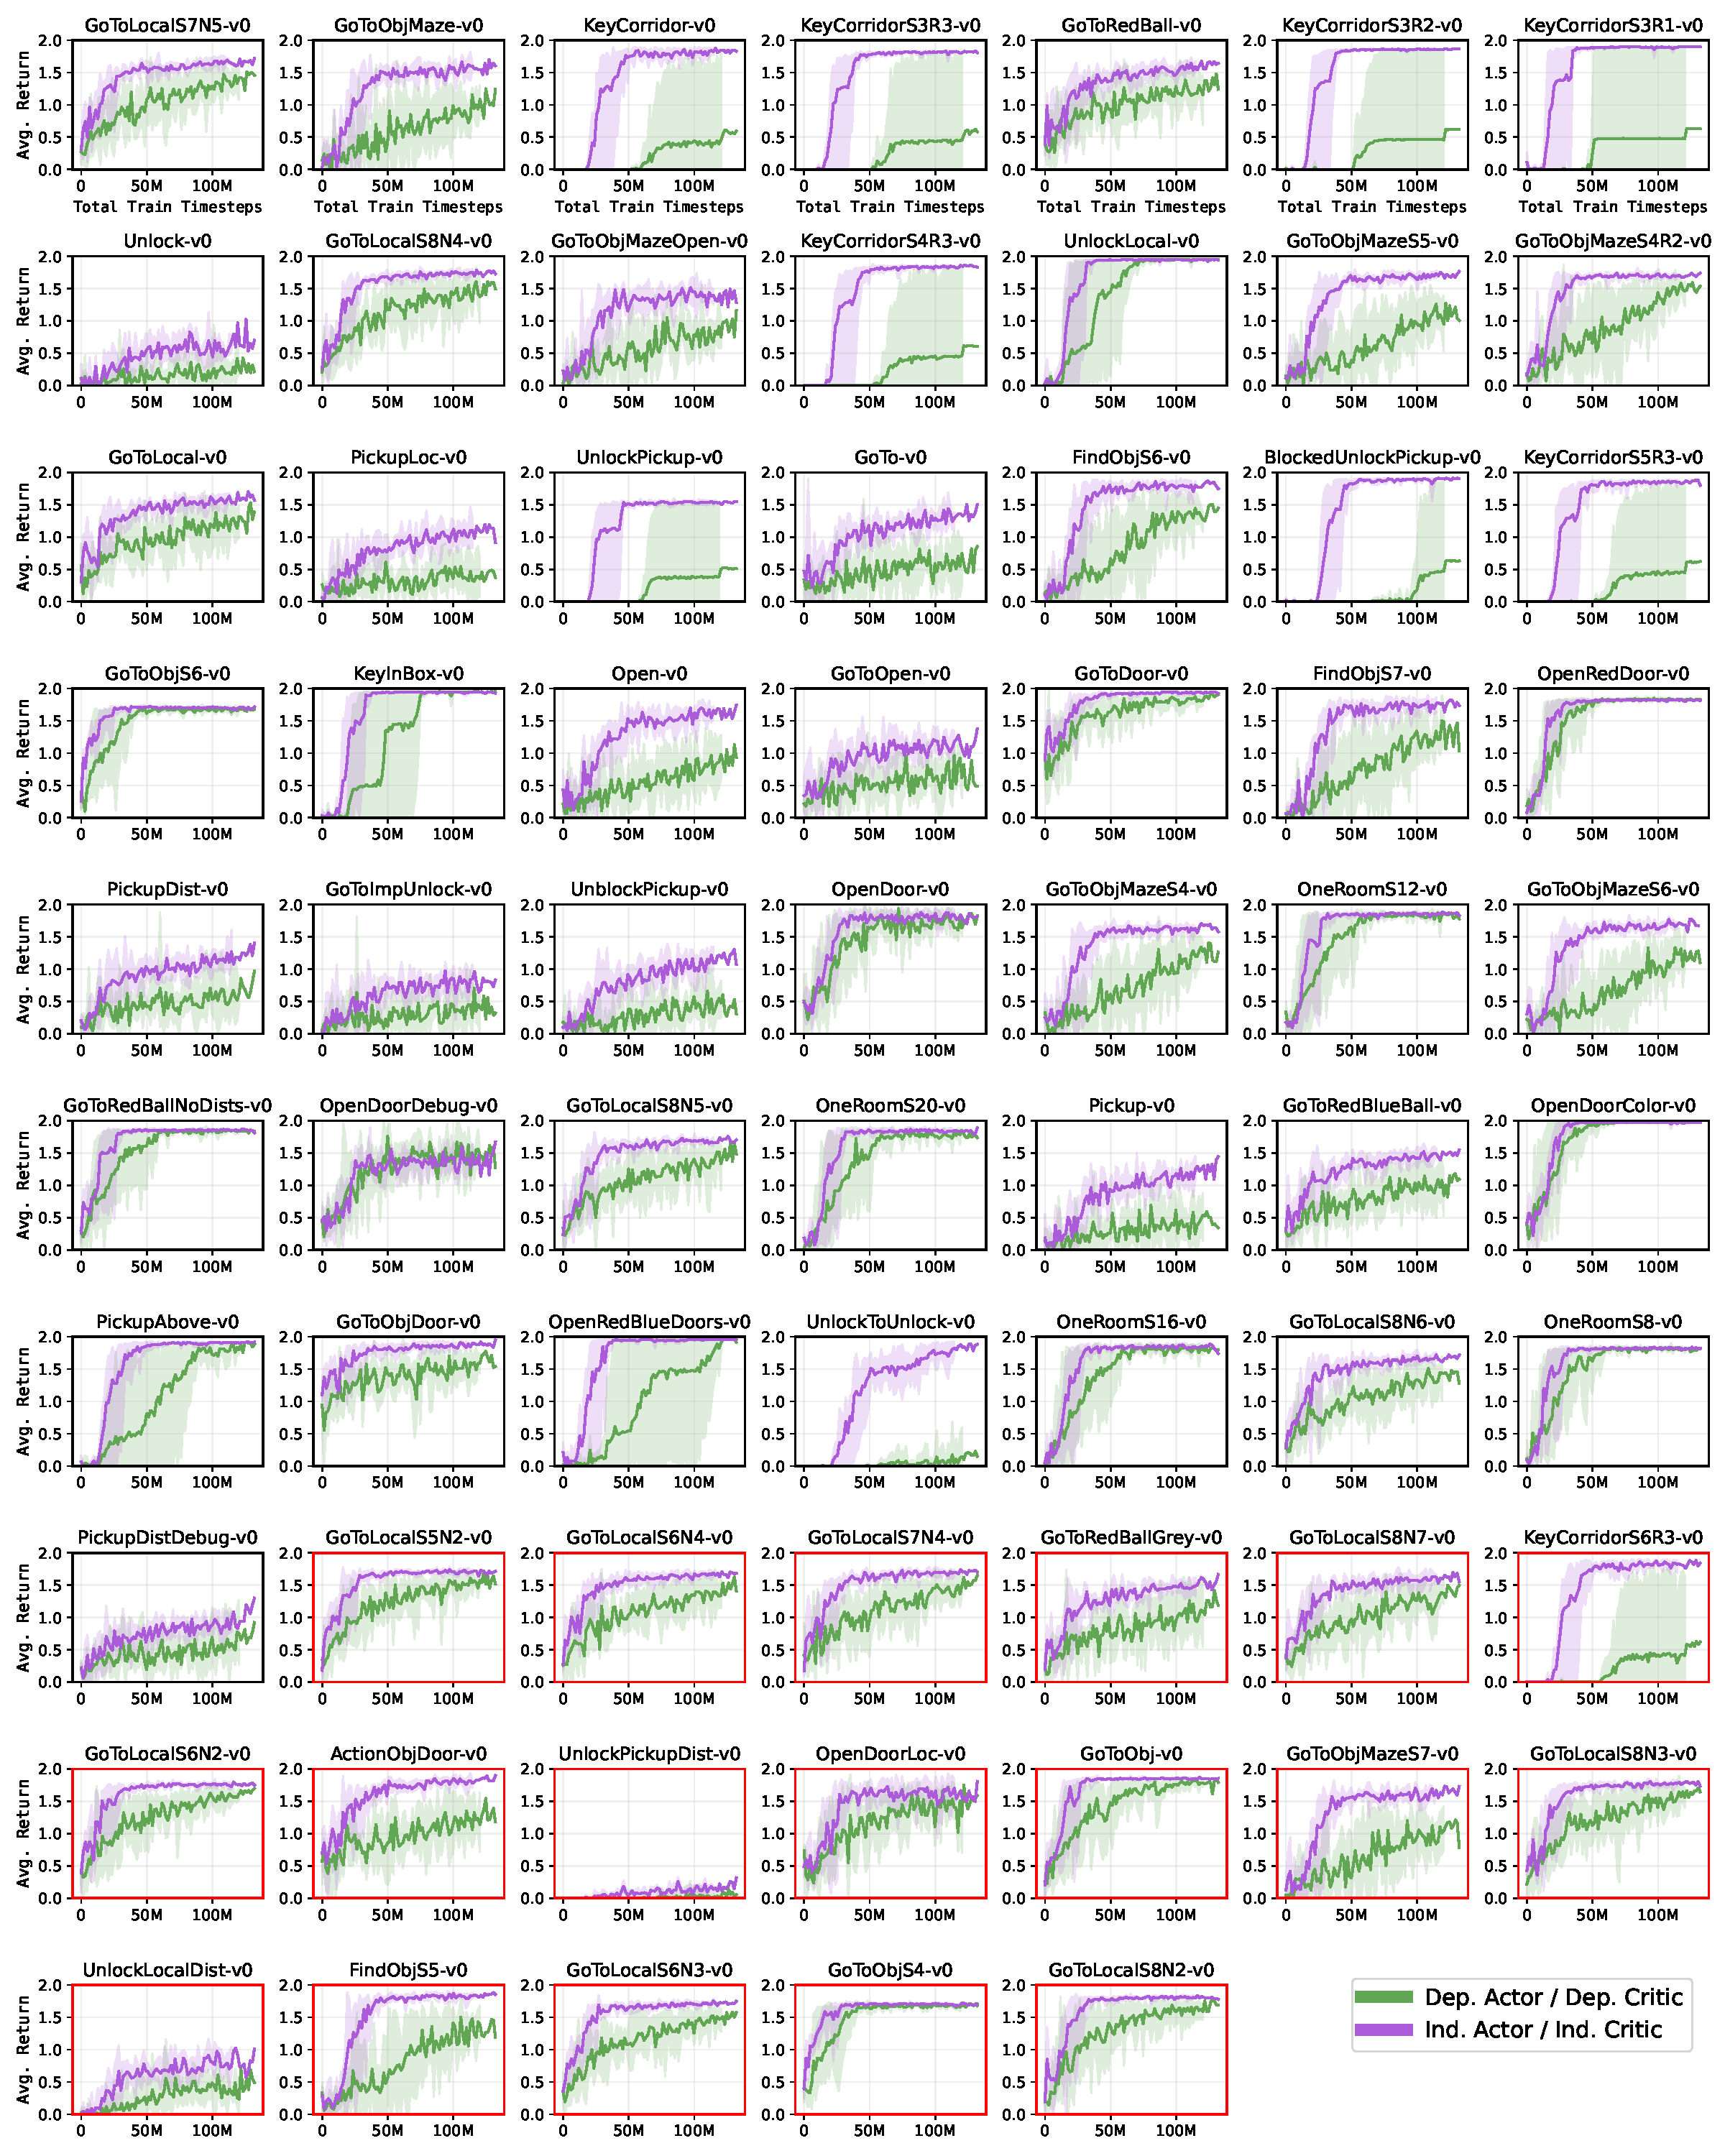
\includegraphics[width=\linewidth]{figures/final/all_babyai_curves.pdf}
    \caption{\textbf{Two-Episode Multi-Task BabyAI.} Held-out test tasks are highlighted in \textcolor{red}{red}. Error bars denote the maximum and minimum value of four random trials.}
    \label{fig:babyai_appendix}
\end{figure}

\begin{figure}[h!]
    \centering
    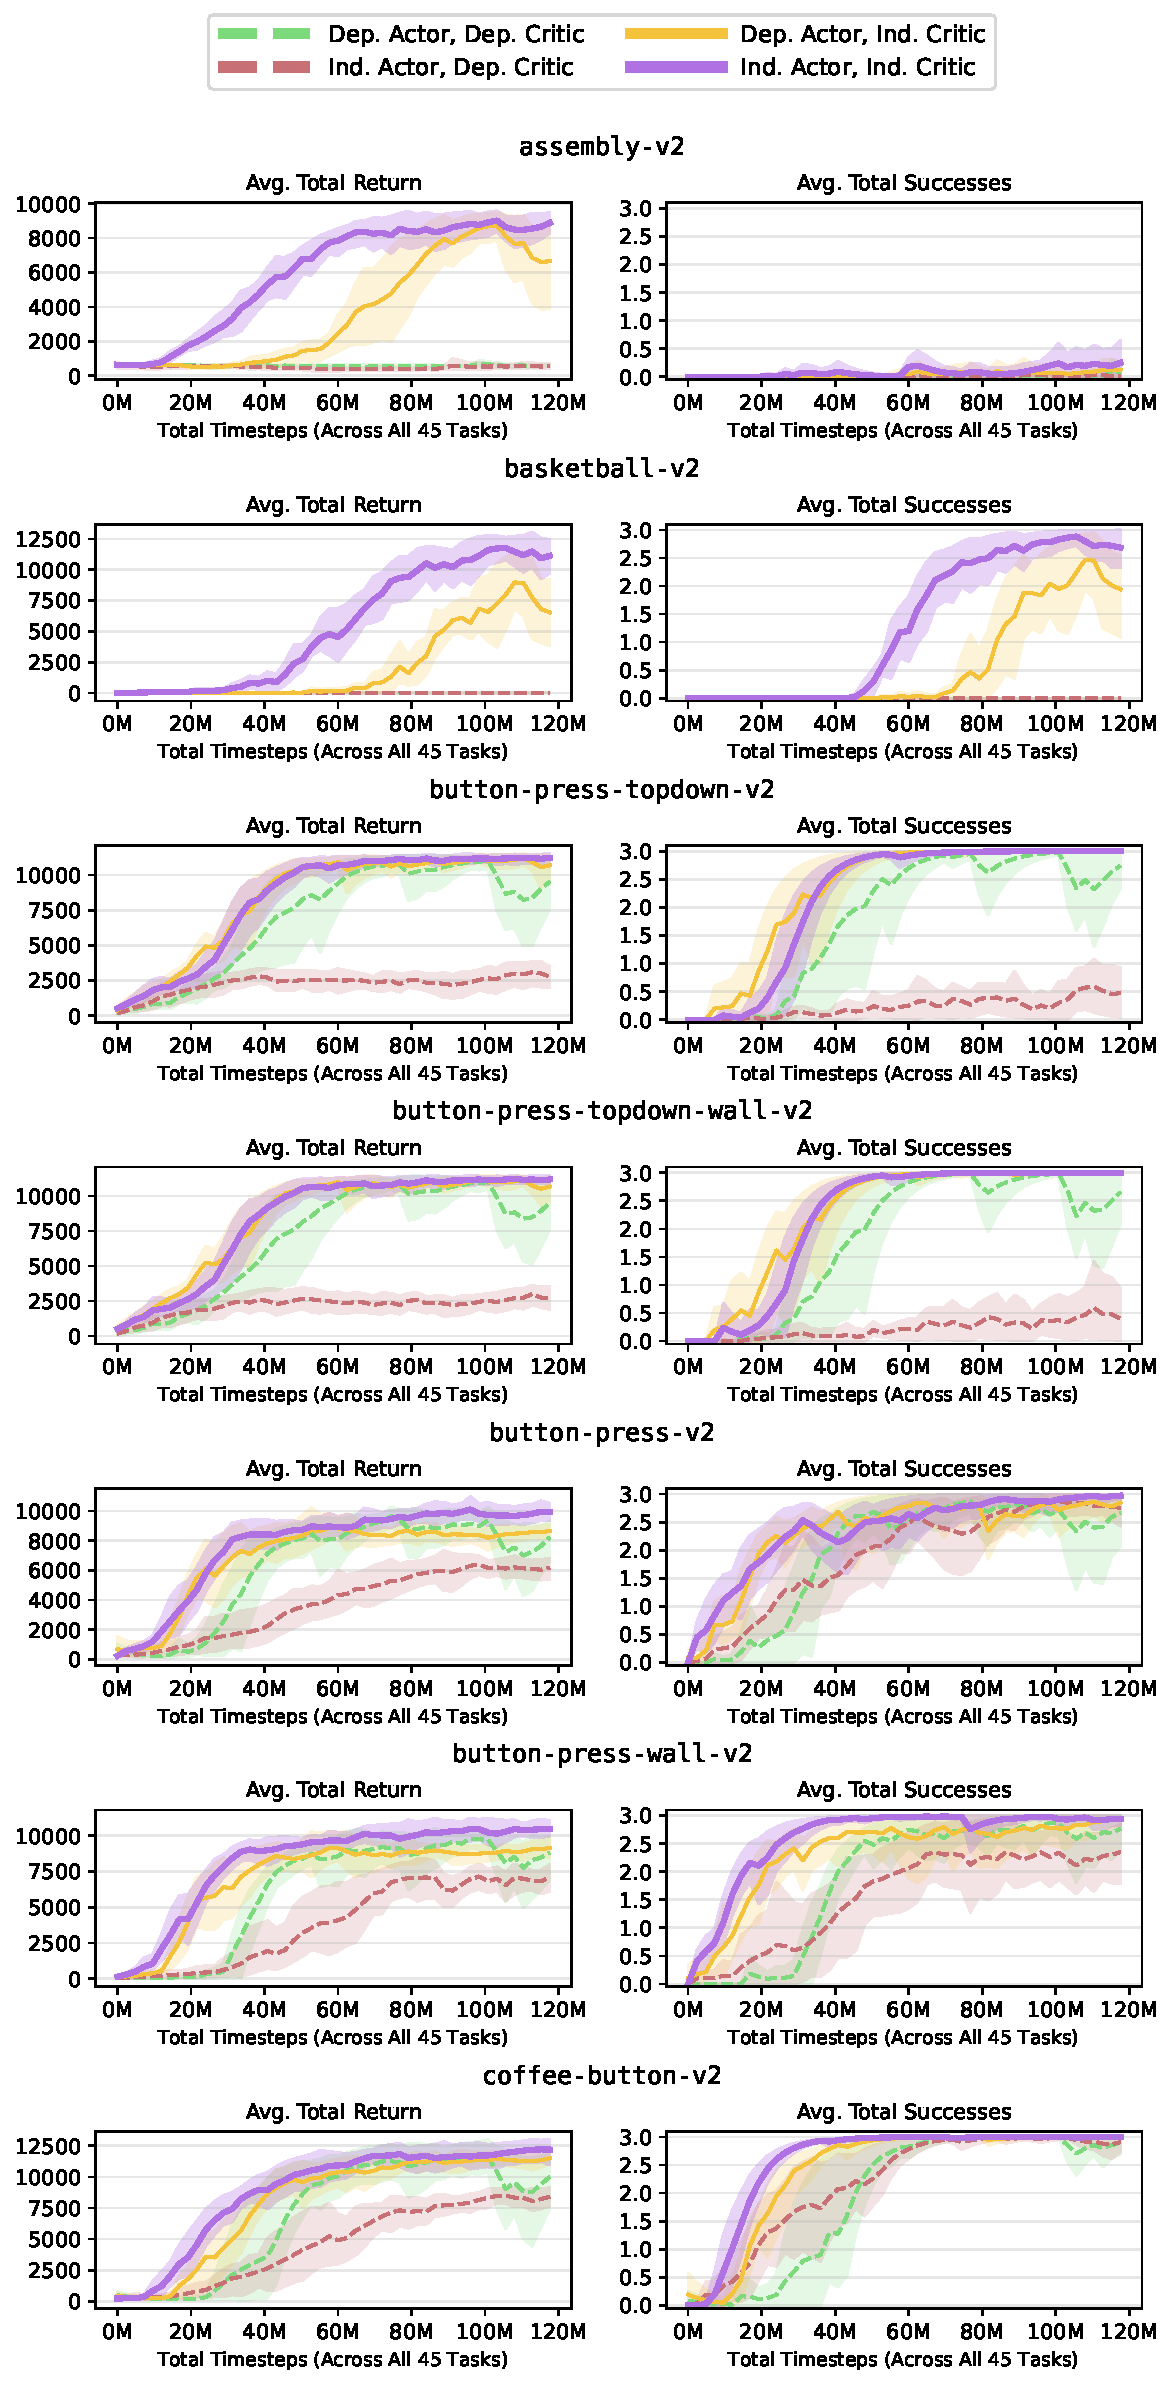
\includegraphics[width=300px]{figures/raw_metaworld_curves/raw_metaworld_curves_page0-2.pdf}
    \caption{\textbf{Three-Episode Meta-World ML45 Learning Curves (Part 1/7)}}
\end{figure}
\newpage

\begin{figure}[h!]
    \centering
    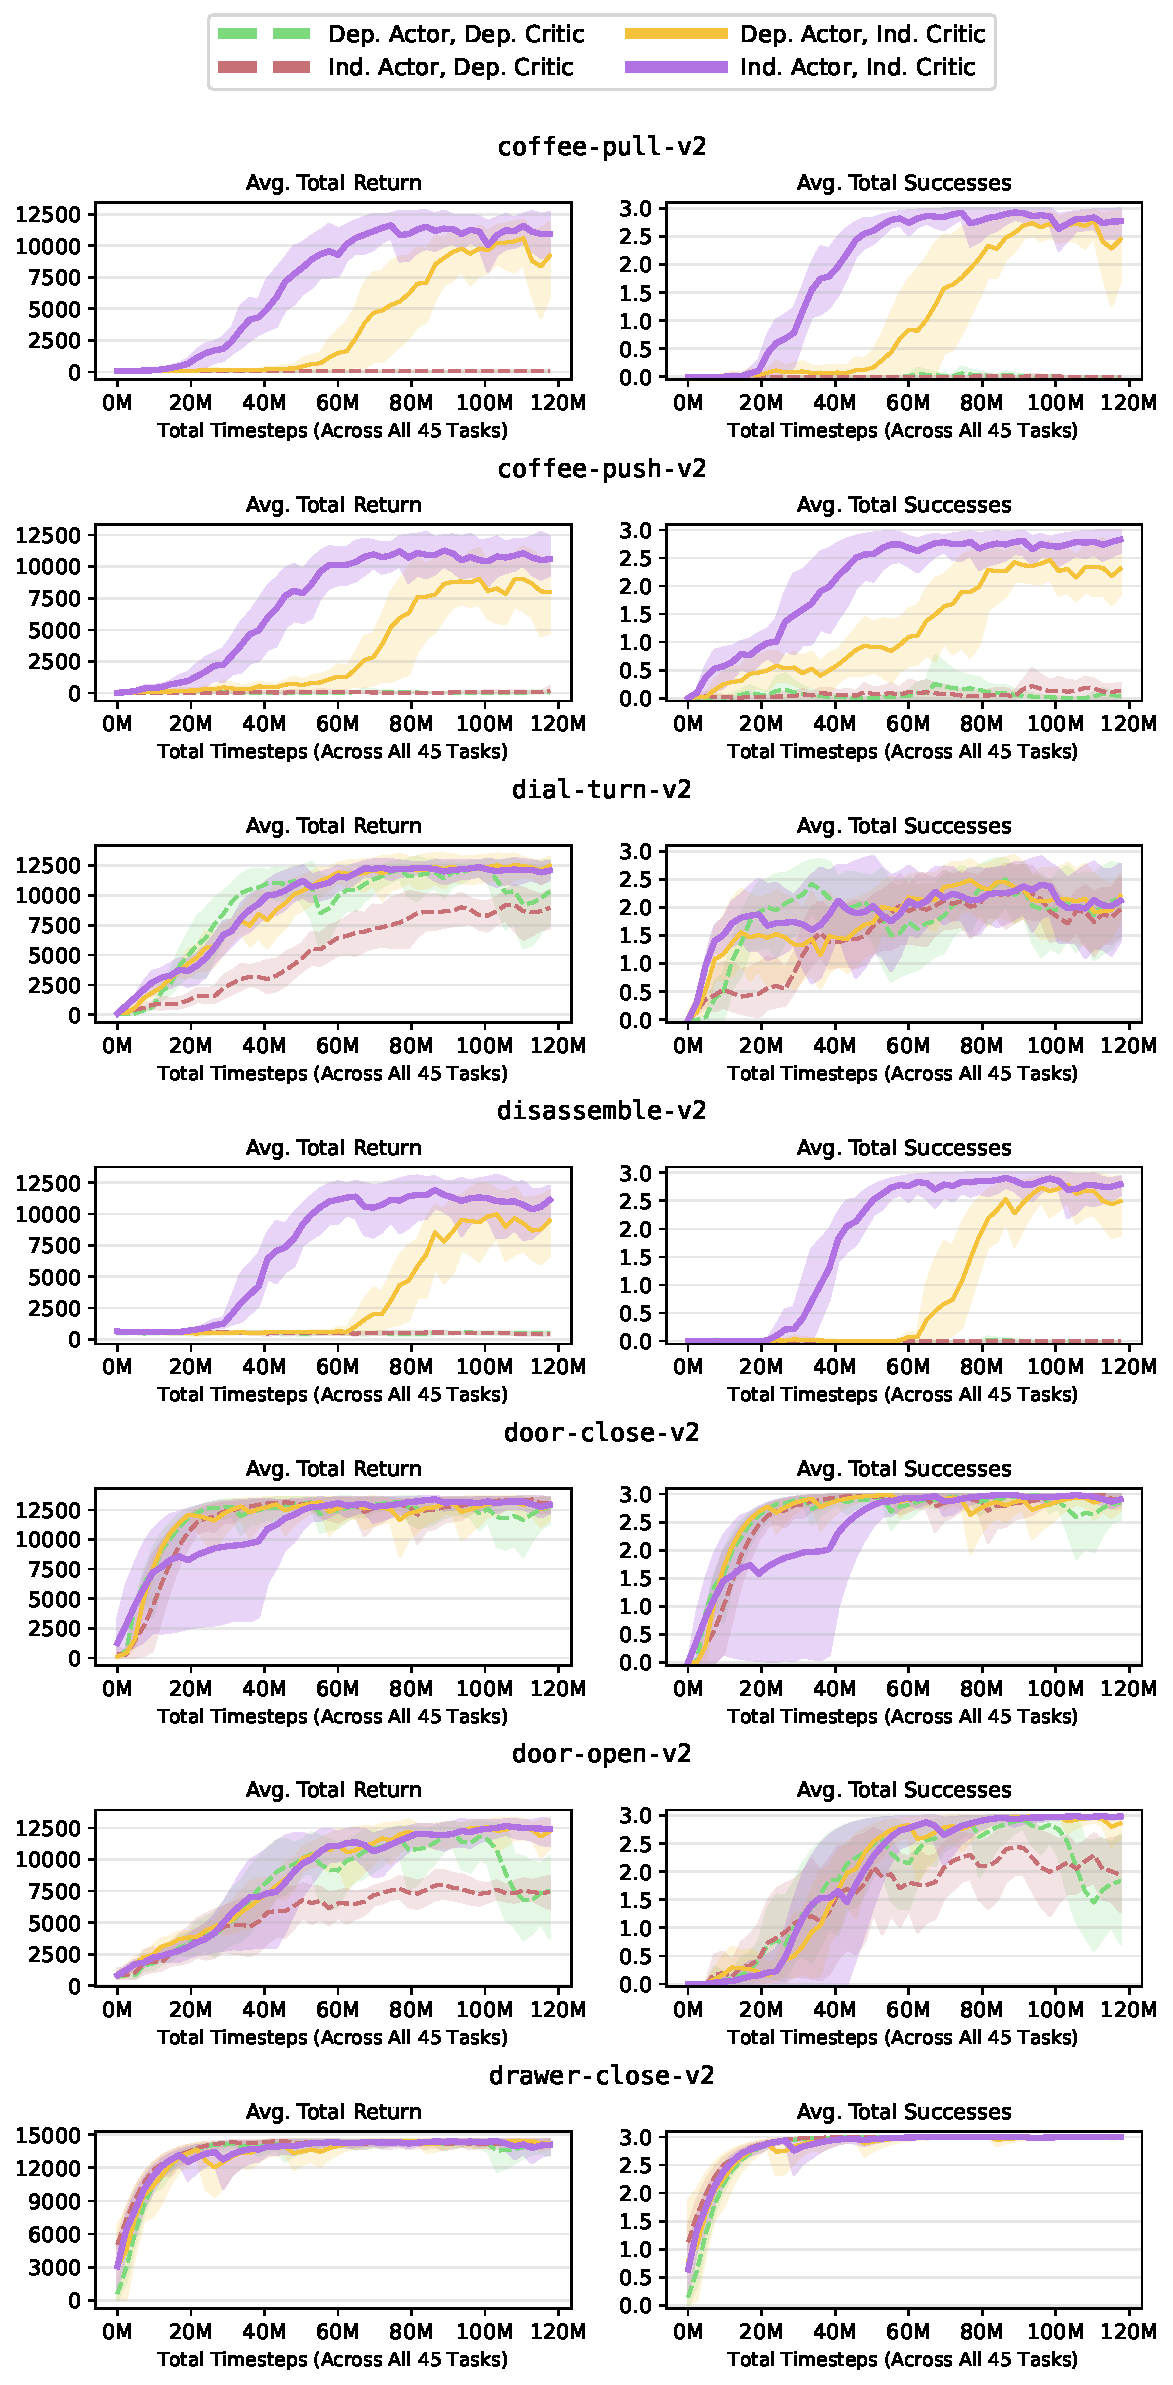
\includegraphics[width=300px]{figures/raw_metaworld_curves/raw_metaworld_curves_page1-2.pdf}
    \caption{\textbf{Three-Episode Meta-World ML45 Learning Curves (Part 2/7)}}
\end{figure}
\newpage

\begin{figure}[h!]
    \centering
    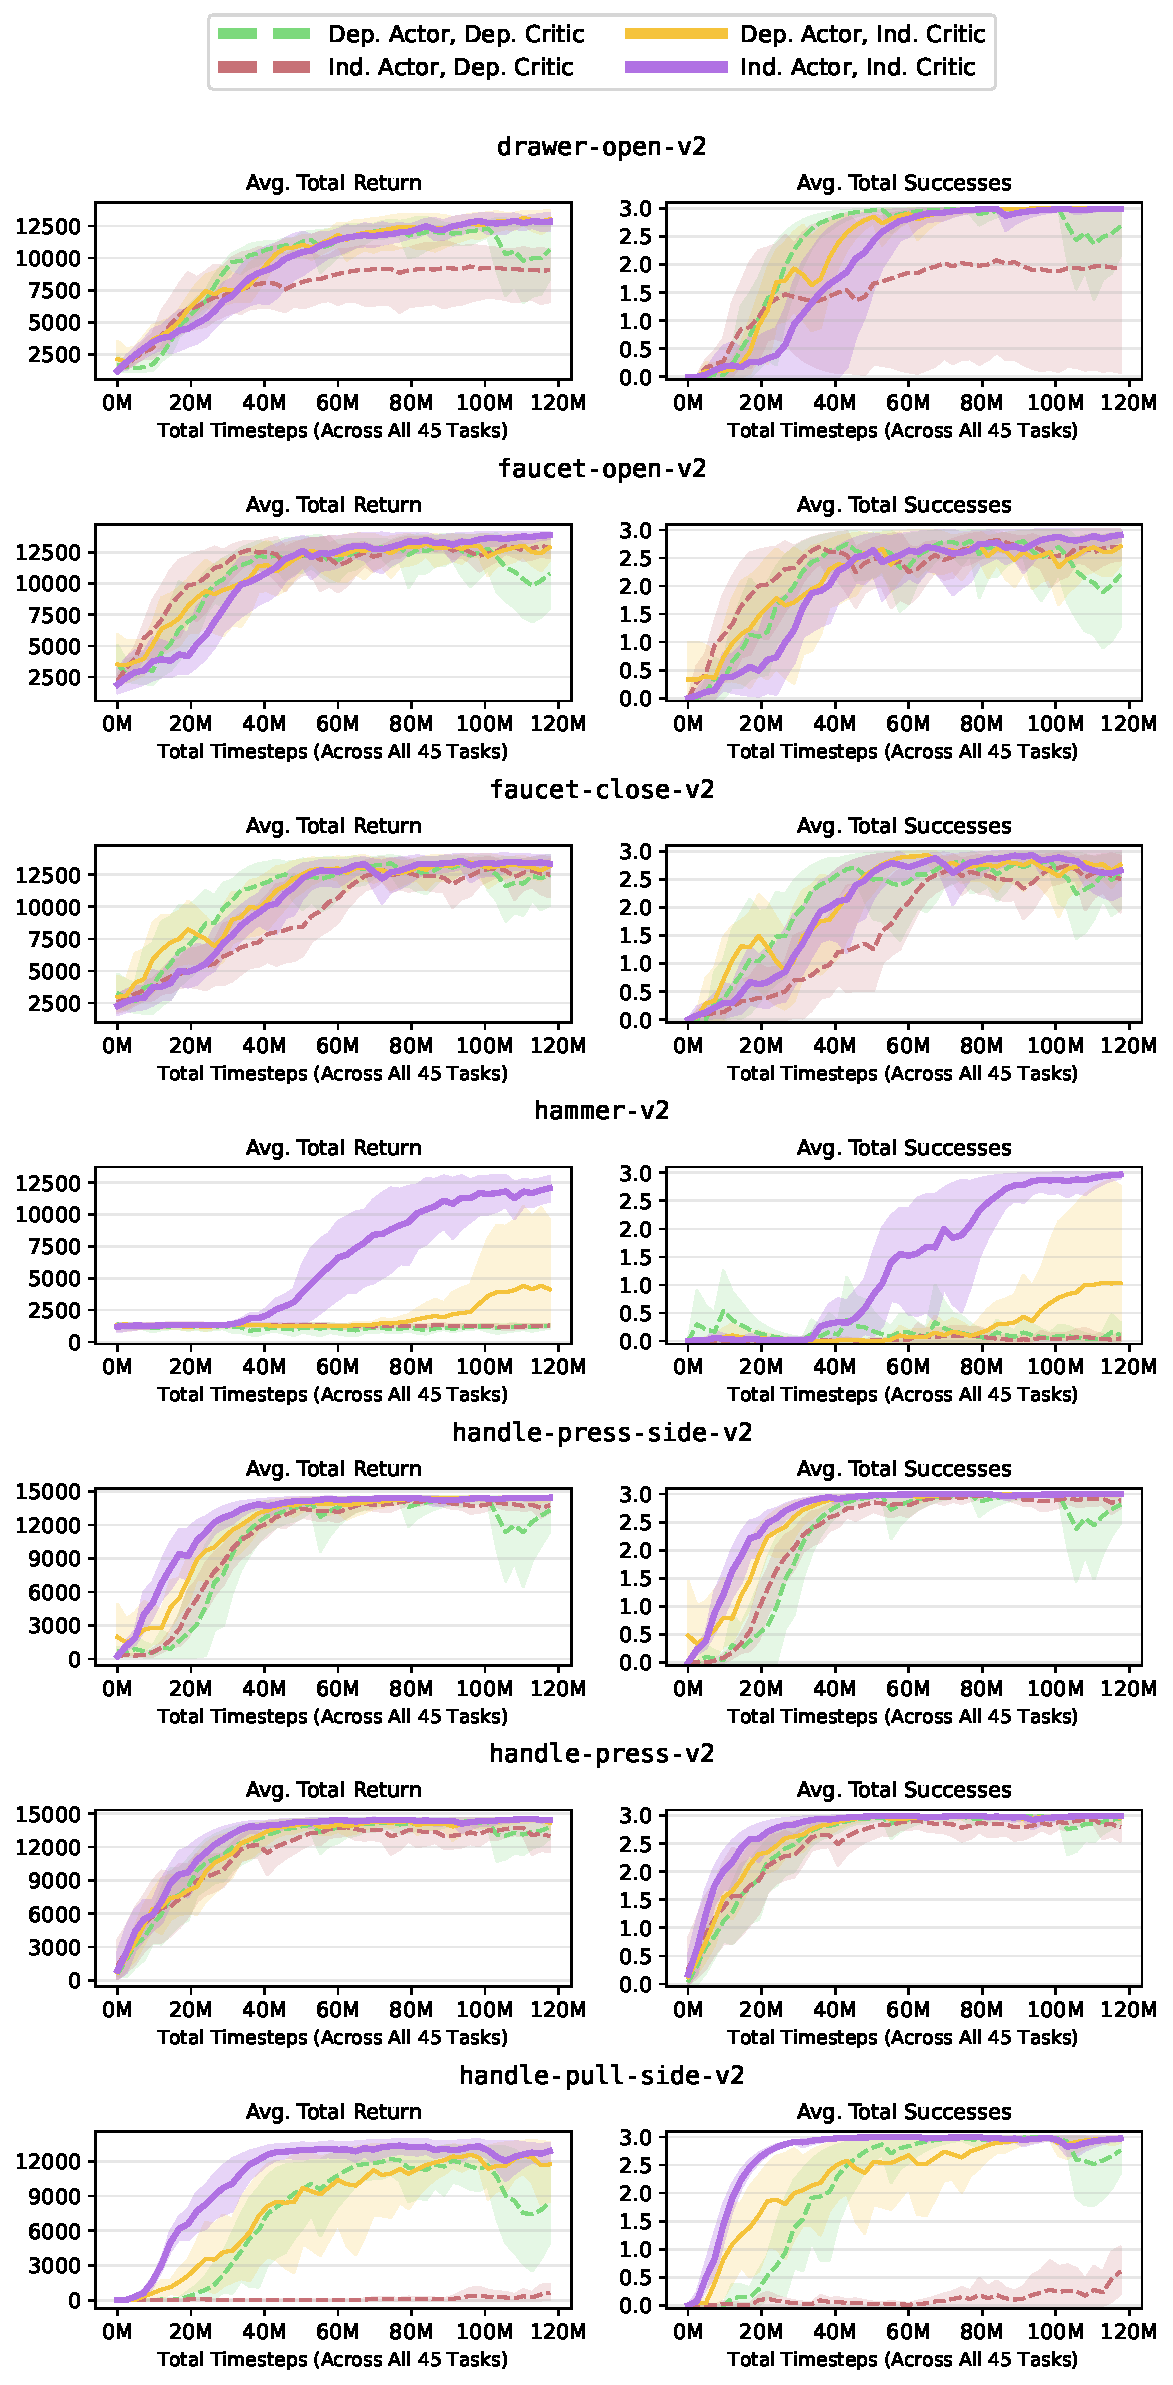
\includegraphics[width=300px]{figures/raw_metaworld_curves/raw_metaworld_curves_page2-5.pdf}
    \caption{\textbf{Three-Episode Meta-World ML45 Learning Curves (Part 3/7)}}
\end{figure}
\newpage

\begin{figure}[h!]
    \centering
    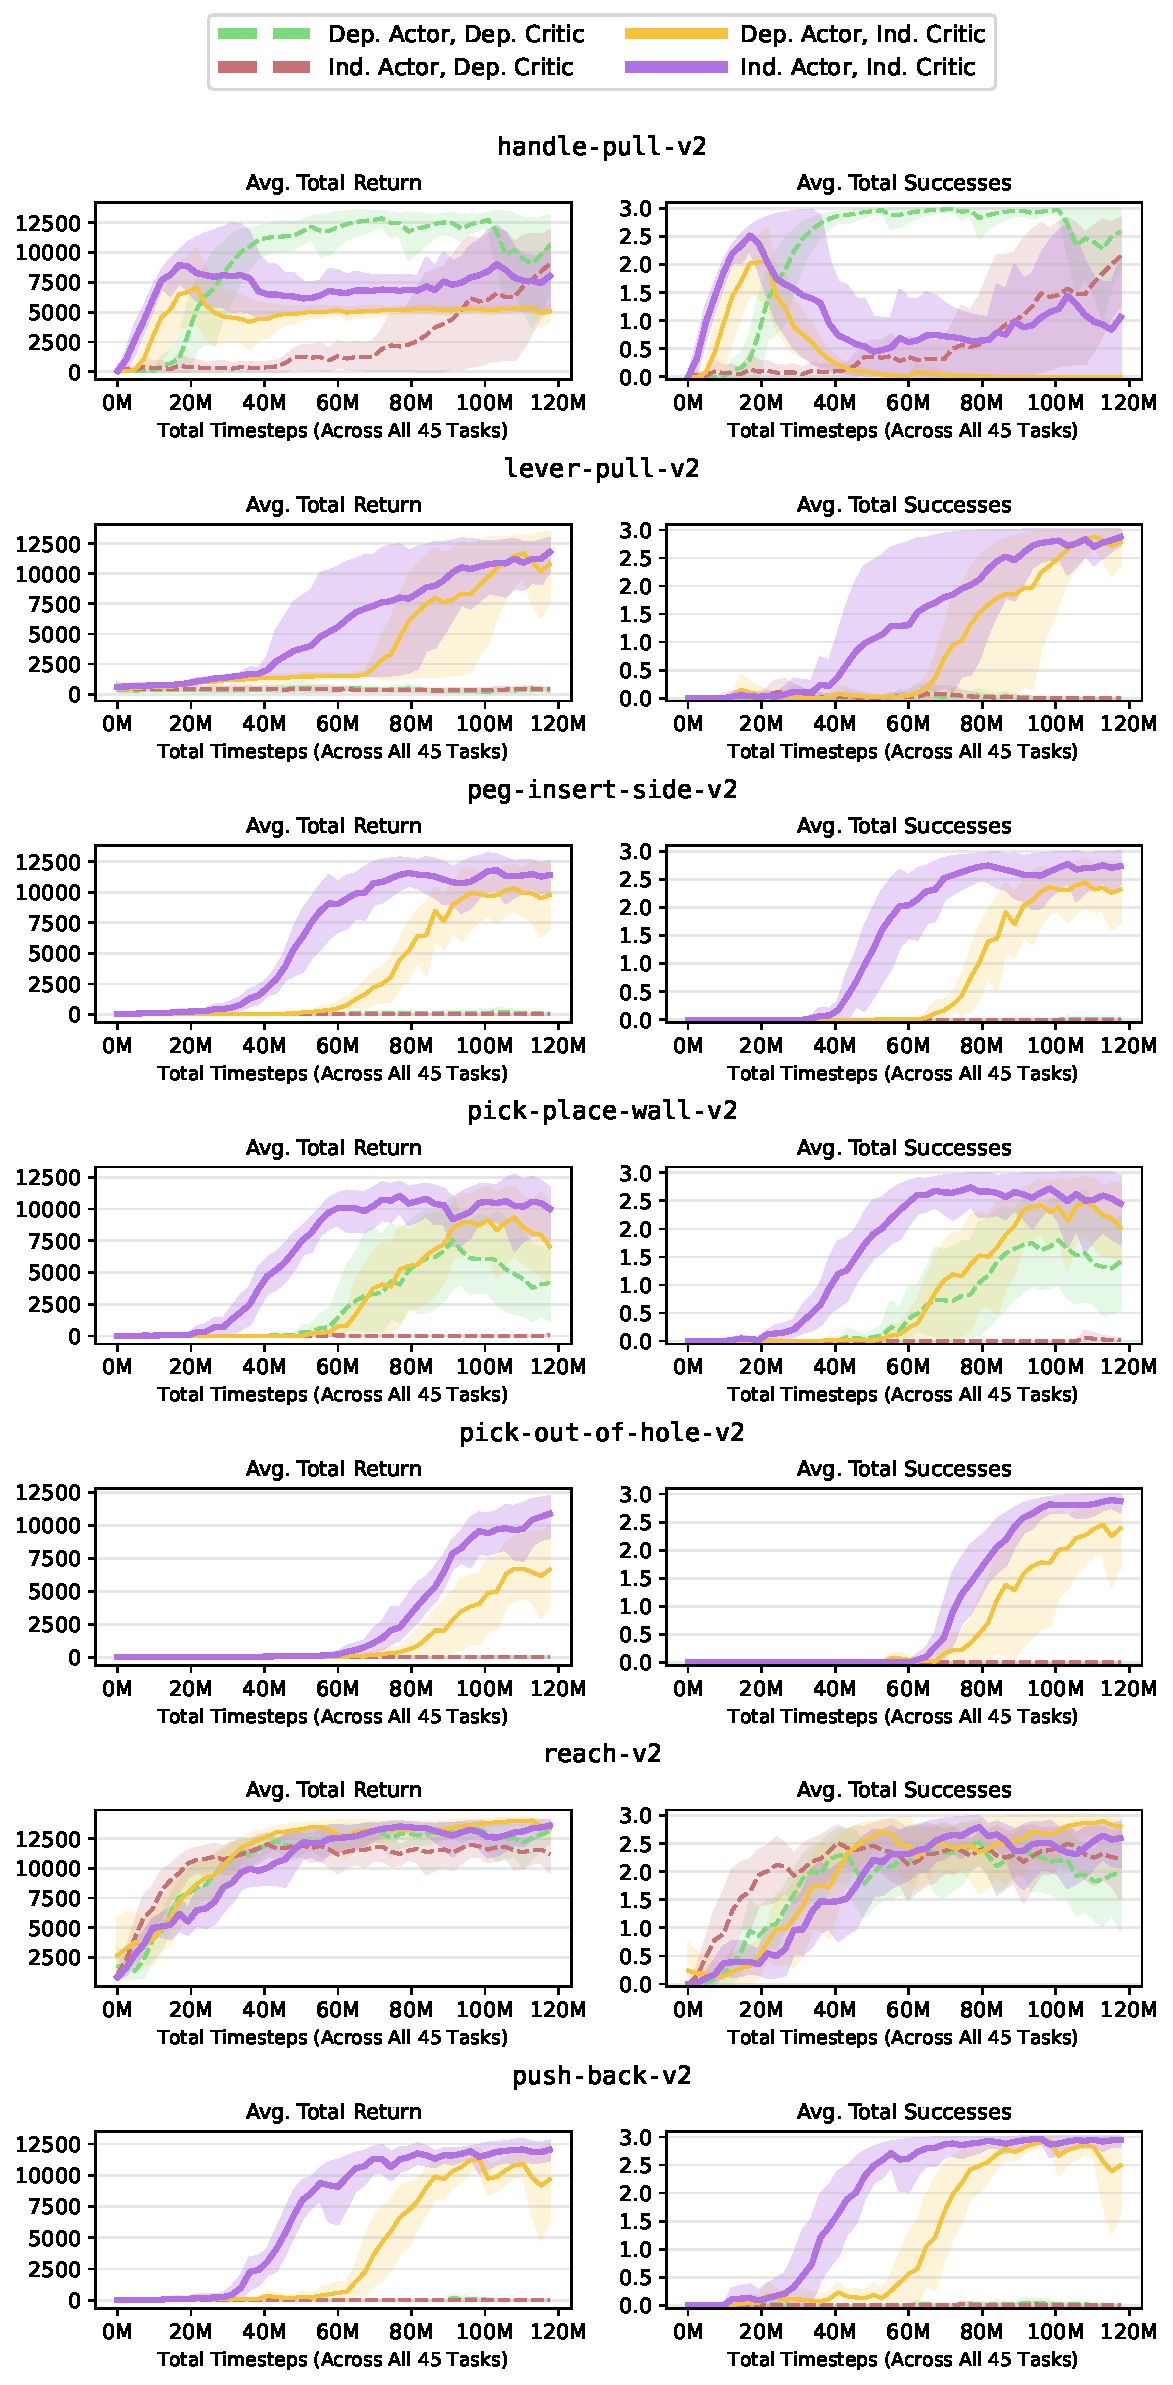
\includegraphics[width=300px]{figures/raw_metaworld_curves/raw_metaworld_curves_page3-3.pdf}
    \caption{\textbf{Three-Episode Meta-World ML45 Learning Curves (Part 4/7)}}
\end{figure}
\newpage

\begin{figure}[h!]
    \centering
    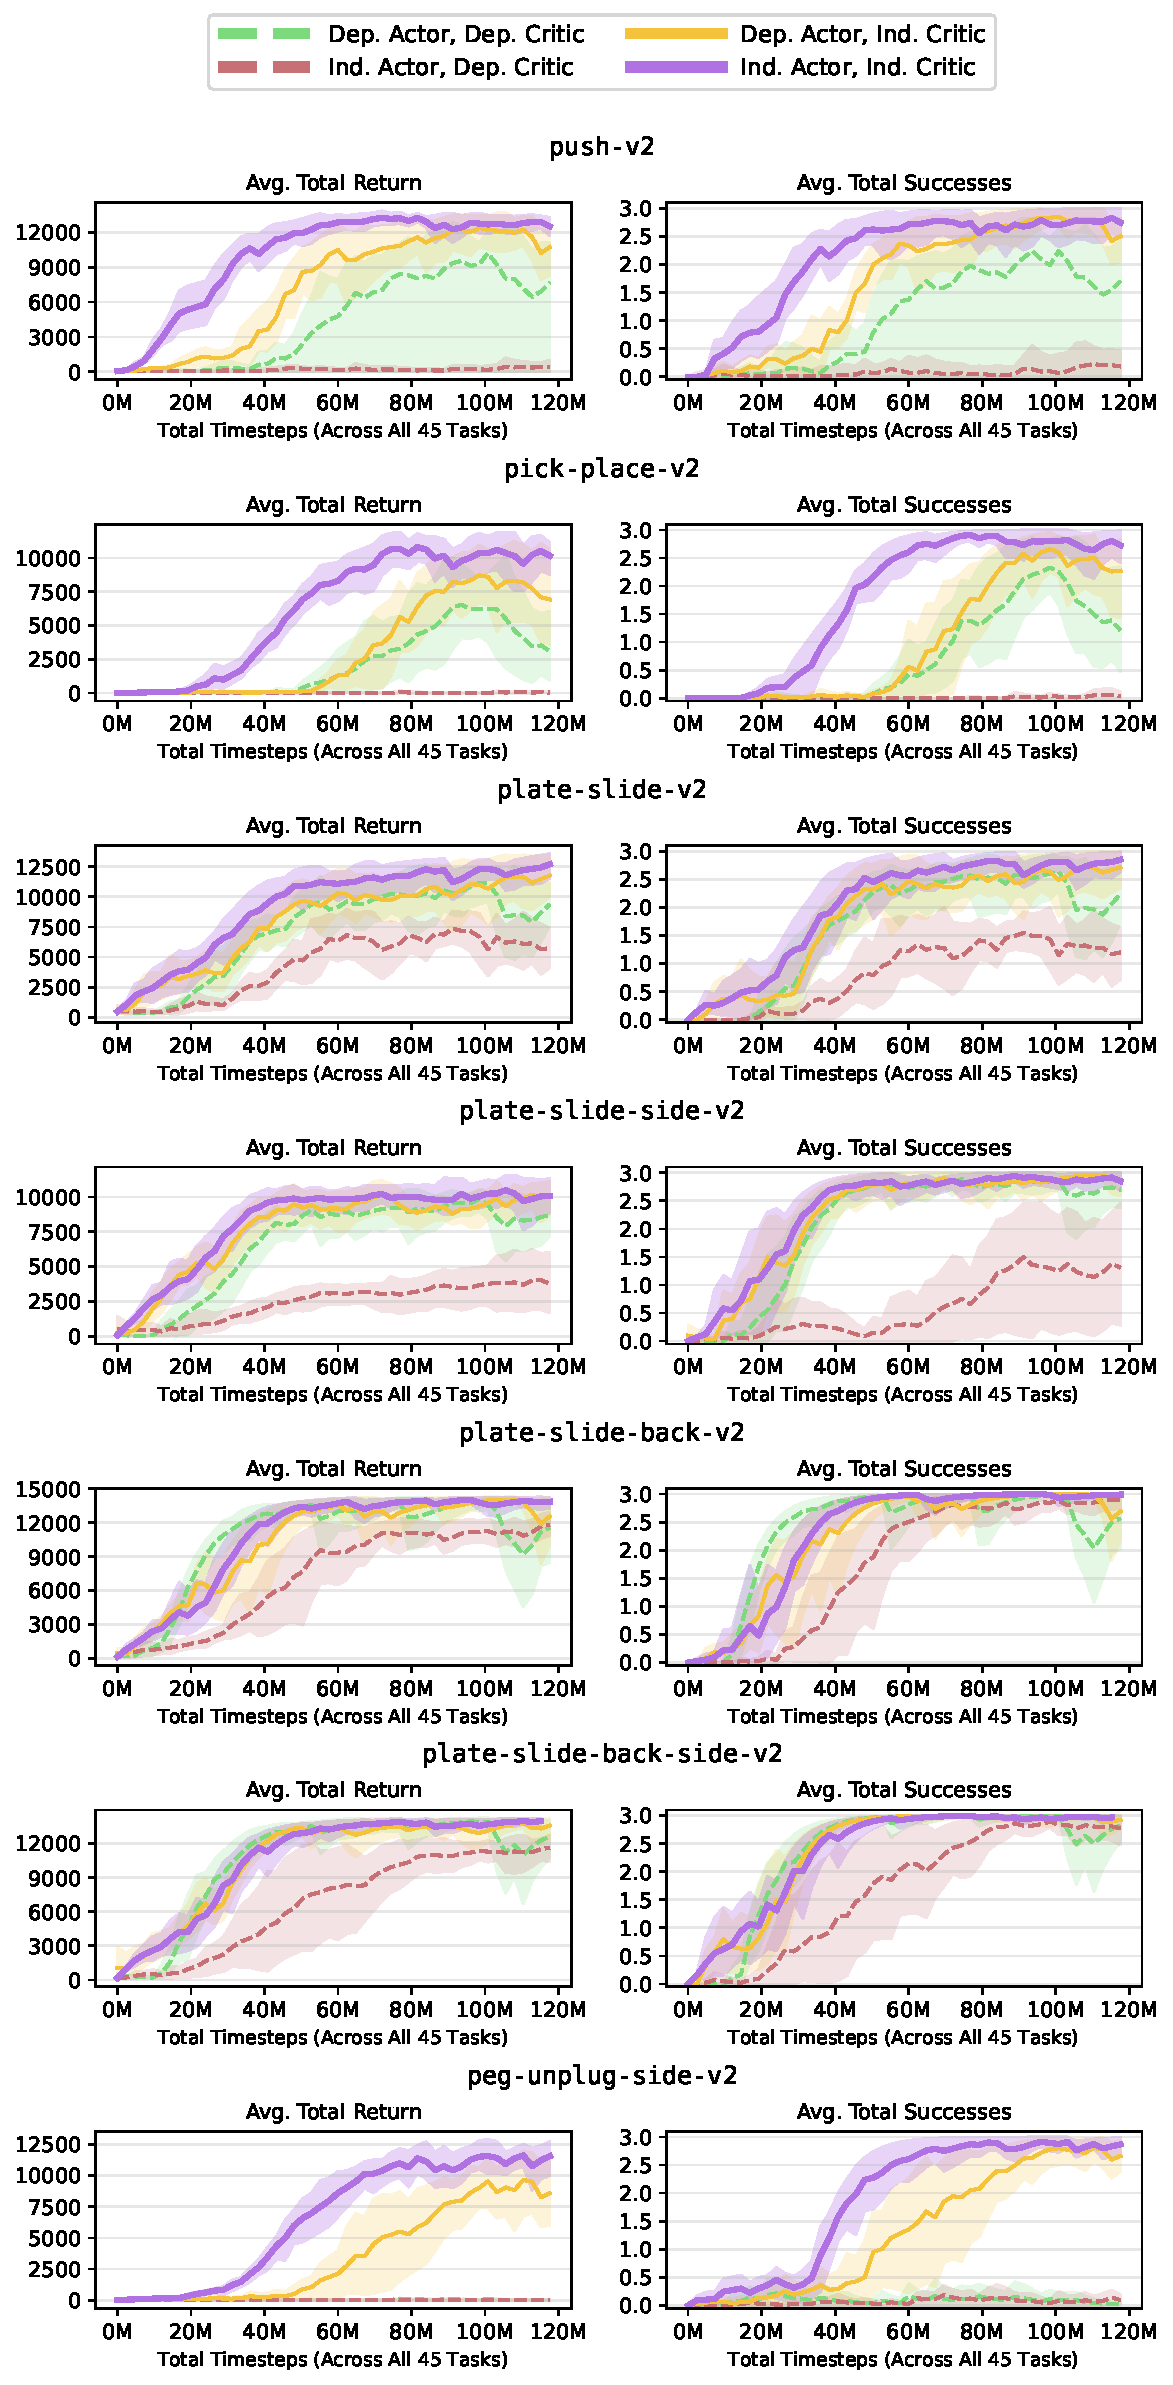
\includegraphics[width=300px]{figures/raw_metaworld_curves/raw_metaworld_curves_page4-2.pdf}
    \caption{\textbf{Three-Episode Meta-World ML45 Learning Curves (Part 5/7)}}
\end{figure}
\newpage


\begin{figure}[h!]
    \centering
    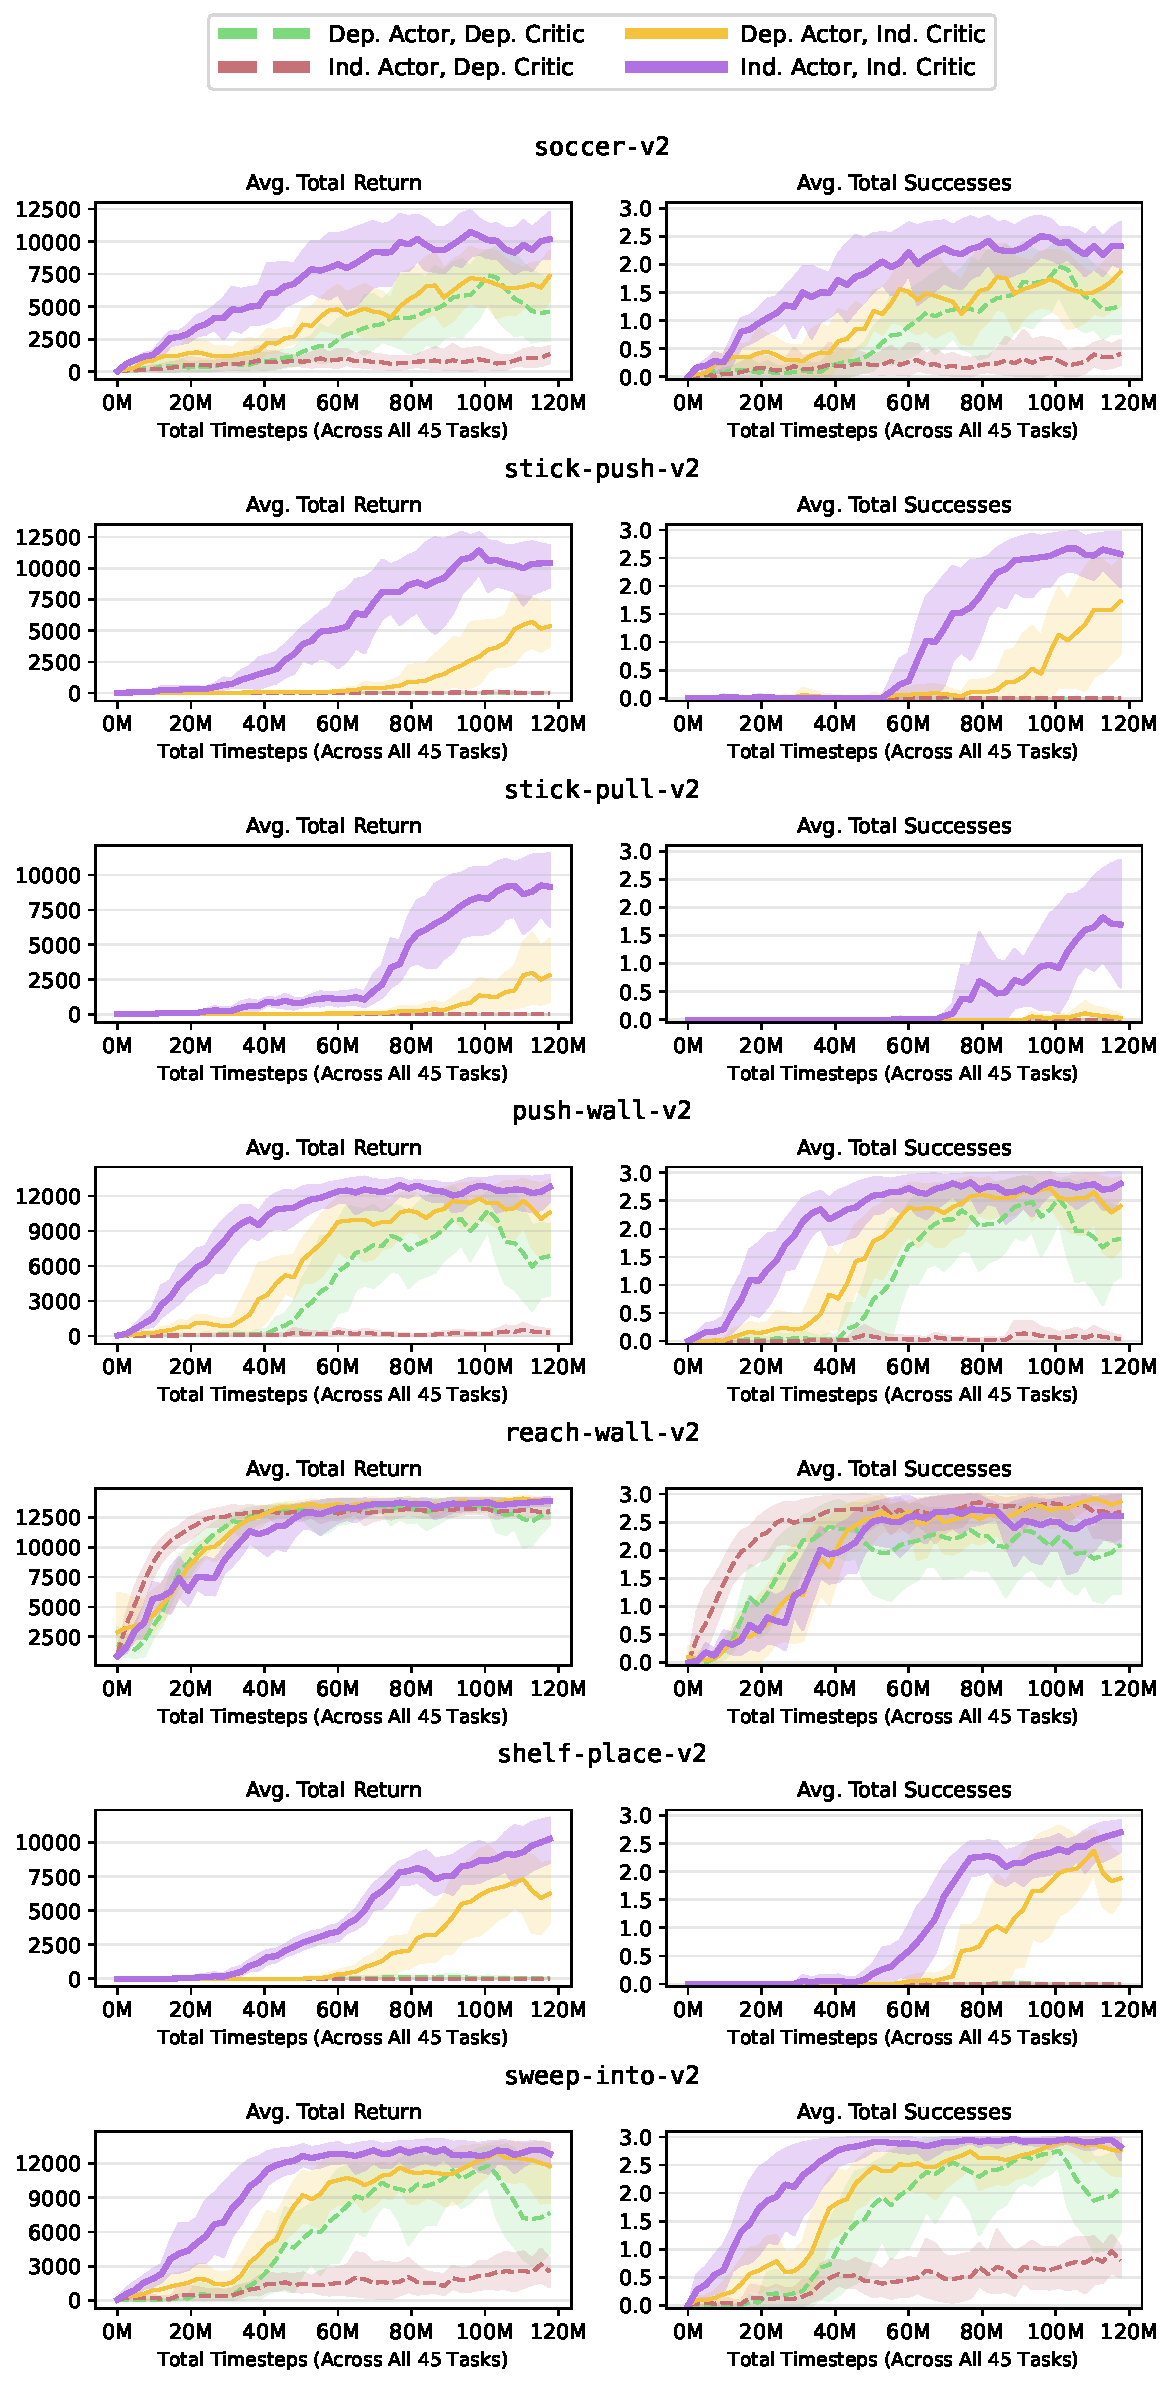
\includegraphics[width=300px]{figures/raw_metaworld_curves/raw_metaworld_curves_page5-3.pdf}
    \caption{\textbf{Three-Episode Meta-World ML45 Learning Curves (Part 6/7)}}
\end{figure}
\newpage

\begin{figure}[h!]
    \centering
    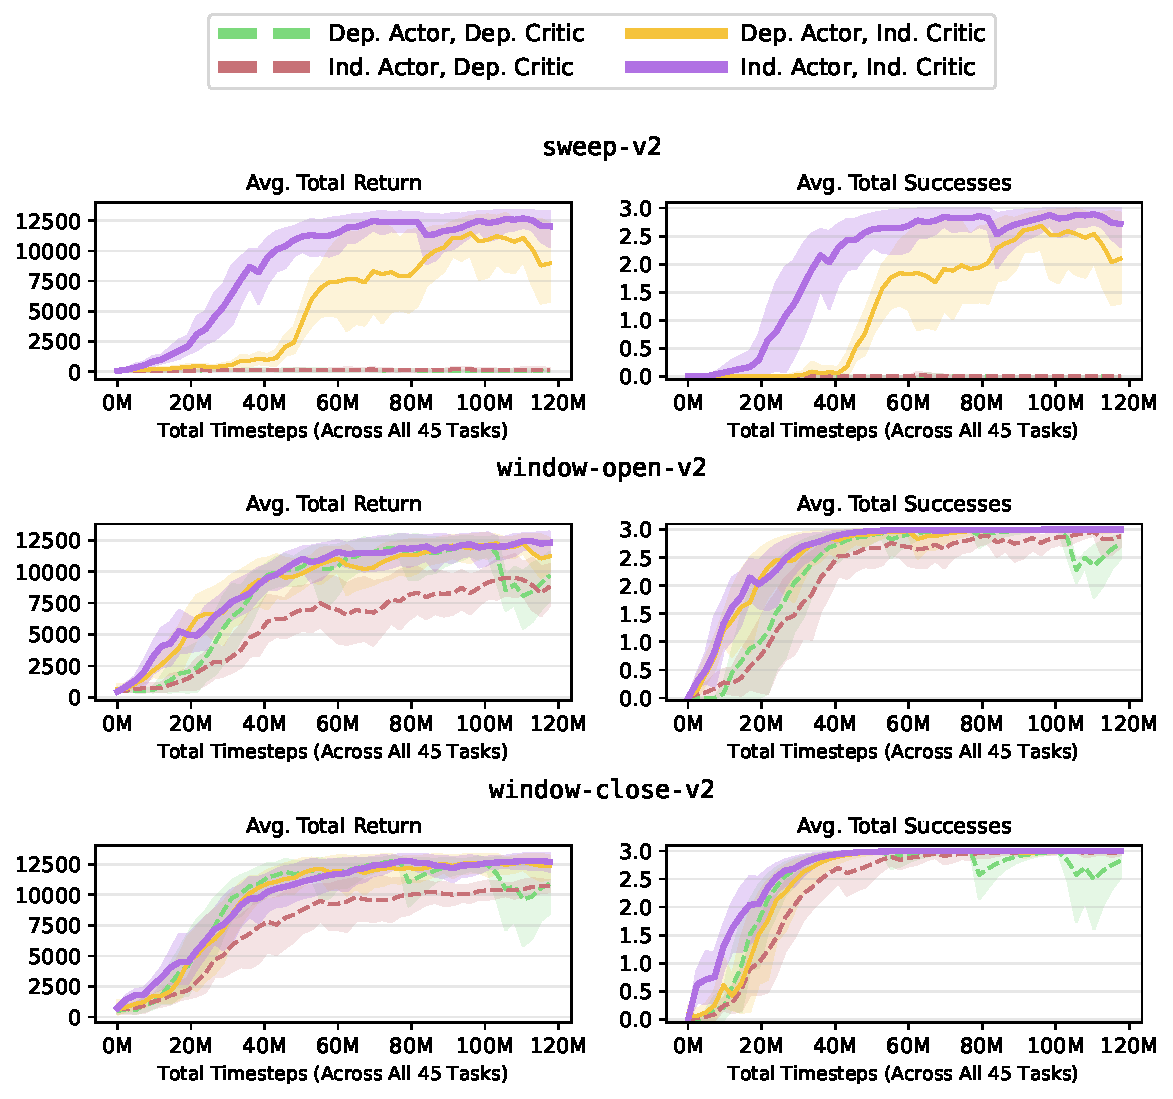
\includegraphics[width=330px]{figures/raw_metaworld_curves/raw_metaworld_curves_page6-4.pdf}
    \caption{\textbf{Three-Episode Meta-World ML45 Learning Curves (Part 7/7)}}
\end{figure}
\newpage

%\paragraph{Gym Retro.} The multi-console Mario environment (Figure \ref{fig:mario-result}) is built on \texttt{stable-retro} \cite{stable-retro}. Similar to the multi-task POPGym setup, we create a padded action space of $12$ MultiBinary actions. Each index of a multibinary action corresponds to pressing a button on a game controller. We indicate the current game console with a thin colored border around the outside of the screen. Each game is played at a resolution of $(84, 84)$ pixels with a frame skip of $8$ and a maximum time limit of $8$ minutes.

%Section \ref{sec:background} mentions large-scale game-playing as a potential application of meta-RL that runs into multi-task optimization challenges at small scales. The most promising opportunity for making research progress towards this goal might be Gym Retro \cite{nichol2018gotta, stable-retro}.

% \begin{figure}[h!]
%     \centering
%     
\includegraphics[width=\linewidth]{figures/mario_appendix_result.pdf}
%     \caption{\textbf{Mario in Gym Retro.} We train multi-task agents on $40$ start states from $4$ Super Mario games in Gym Retro \cite{nichol2018gotta, stable-retro}. Similar to the multi-task POPGym setup, we create a padded action space of $12$ MultiBinary actions. Each index of a multibinary action corresponds to pressing a button on a game controller. We indicate the current game console with a thin colored border around the outside of the screen. Each game is played at a resolution of $(84, 84)$ pixels with a frame skip of $8$ and a maximum time limit of $8$ minutes. in SuperMarioBros-Nes are plotted against a human reference baseline. Results in the other three games are plotted according to the relative gain of ``Ind. / Ind.'' (II) over ``Ind. / Dep.`` (ID), ($(\text{II} - \text{ID}) / |\text{ID}|$).}
%     \label{fig:mario-result}
% \end{figure}